% Options for packages loaded elsewhere
\PassOptionsToPackage{unicode}{hyperref}
\PassOptionsToPackage{hyphens}{url}
\PassOptionsToPackage{dvipsnames,svgnames,x11names}{xcolor}
%
\documentclass[
  letterpaper,
  DIV=11,
  numbers=noendperiod]{scrartcl}

\usepackage{amsmath,amssymb}
\usepackage{lmodern}
\usepackage{iftex}
\ifPDFTeX
  \usepackage[T1]{fontenc}
  \usepackage[utf8]{inputenc}
  \usepackage{textcomp} % provide euro and other symbols
\else % if luatex or xetex
  \usepackage{unicode-math}
  \defaultfontfeatures{Scale=MatchLowercase}
  \defaultfontfeatures[\rmfamily]{Ligatures=TeX,Scale=1}
\fi
% Use upquote if available, for straight quotes in verbatim environments
\IfFileExists{upquote.sty}{\usepackage{upquote}}{}
\IfFileExists{microtype.sty}{% use microtype if available
  \usepackage[]{microtype}
  \UseMicrotypeSet[protrusion]{basicmath} % disable protrusion for tt fonts
}{}
\makeatletter
\@ifundefined{KOMAClassName}{% if non-KOMA class
  \IfFileExists{parskip.sty}{%
    \usepackage{parskip}
  }{% else
    \setlength{\parindent}{0pt}
    \setlength{\parskip}{6pt plus 2pt minus 1pt}}
}{% if KOMA class
  \KOMAoptions{parskip=half}}
\makeatother
\usepackage{xcolor}
\setlength{\emergencystretch}{3em} % prevent overfull lines
\setcounter{secnumdepth}{-\maxdimen} % remove section numbering
% Make \paragraph and \subparagraph free-standing
\ifx\paragraph\undefined\else
  \let\oldparagraph\paragraph
  \renewcommand{\paragraph}[1]{\oldparagraph{#1}\mbox{}}
\fi
\ifx\subparagraph\undefined\else
  \let\oldsubparagraph\subparagraph
  \renewcommand{\subparagraph}[1]{\oldsubparagraph{#1}\mbox{}}
\fi

\usepackage{color}
\usepackage{fancyvrb}
\newcommand{\VerbBar}{|}
\newcommand{\VERB}{\Verb[commandchars=\\\{\}]}
\DefineVerbatimEnvironment{Highlighting}{Verbatim}{commandchars=\\\{\}}
% Add ',fontsize=\small' for more characters per line
\usepackage{framed}
\definecolor{shadecolor}{RGB}{241,243,245}
\newenvironment{Shaded}{\begin{snugshade}}{\end{snugshade}}
\newcommand{\AlertTok}[1]{\textcolor[rgb]{0.68,0.00,0.00}{#1}}
\newcommand{\AnnotationTok}[1]{\textcolor[rgb]{0.37,0.37,0.37}{#1}}
\newcommand{\AttributeTok}[1]{\textcolor[rgb]{0.40,0.45,0.13}{#1}}
\newcommand{\BaseNTok}[1]{\textcolor[rgb]{0.68,0.00,0.00}{#1}}
\newcommand{\BuiltInTok}[1]{\textcolor[rgb]{0.00,0.23,0.31}{#1}}
\newcommand{\CharTok}[1]{\textcolor[rgb]{0.13,0.47,0.30}{#1}}
\newcommand{\CommentTok}[1]{\textcolor[rgb]{0.37,0.37,0.37}{#1}}
\newcommand{\CommentVarTok}[1]{\textcolor[rgb]{0.37,0.37,0.37}{\textit{#1}}}
\newcommand{\ConstantTok}[1]{\textcolor[rgb]{0.56,0.35,0.01}{#1}}
\newcommand{\ControlFlowTok}[1]{\textcolor[rgb]{0.00,0.23,0.31}{#1}}
\newcommand{\DataTypeTok}[1]{\textcolor[rgb]{0.68,0.00,0.00}{#1}}
\newcommand{\DecValTok}[1]{\textcolor[rgb]{0.68,0.00,0.00}{#1}}
\newcommand{\DocumentationTok}[1]{\textcolor[rgb]{0.37,0.37,0.37}{\textit{#1}}}
\newcommand{\ErrorTok}[1]{\textcolor[rgb]{0.68,0.00,0.00}{#1}}
\newcommand{\ExtensionTok}[1]{\textcolor[rgb]{0.00,0.23,0.31}{#1}}
\newcommand{\FloatTok}[1]{\textcolor[rgb]{0.68,0.00,0.00}{#1}}
\newcommand{\FunctionTok}[1]{\textcolor[rgb]{0.28,0.35,0.67}{#1}}
\newcommand{\ImportTok}[1]{\textcolor[rgb]{0.00,0.46,0.62}{#1}}
\newcommand{\InformationTok}[1]{\textcolor[rgb]{0.37,0.37,0.37}{#1}}
\newcommand{\KeywordTok}[1]{\textcolor[rgb]{0.00,0.23,0.31}{#1}}
\newcommand{\NormalTok}[1]{\textcolor[rgb]{0.00,0.23,0.31}{#1}}
\newcommand{\OperatorTok}[1]{\textcolor[rgb]{0.37,0.37,0.37}{#1}}
\newcommand{\OtherTok}[1]{\textcolor[rgb]{0.00,0.23,0.31}{#1}}
\newcommand{\PreprocessorTok}[1]{\textcolor[rgb]{0.68,0.00,0.00}{#1}}
\newcommand{\RegionMarkerTok}[1]{\textcolor[rgb]{0.00,0.23,0.31}{#1}}
\newcommand{\SpecialCharTok}[1]{\textcolor[rgb]{0.37,0.37,0.37}{#1}}
\newcommand{\SpecialStringTok}[1]{\textcolor[rgb]{0.13,0.47,0.30}{#1}}
\newcommand{\StringTok}[1]{\textcolor[rgb]{0.13,0.47,0.30}{#1}}
\newcommand{\VariableTok}[1]{\textcolor[rgb]{0.07,0.07,0.07}{#1}}
\newcommand{\VerbatimStringTok}[1]{\textcolor[rgb]{0.13,0.47,0.30}{#1}}
\newcommand{\WarningTok}[1]{\textcolor[rgb]{0.37,0.37,0.37}{\textit{#1}}}

\providecommand{\tightlist}{%
  \setlength{\itemsep}{0pt}\setlength{\parskip}{0pt}}\usepackage{longtable,booktabs,array}
\usepackage{calc} % for calculating minipage widths
% Correct order of tables after \paragraph or \subparagraph
\usepackage{etoolbox}
\makeatletter
\patchcmd\longtable{\par}{\if@noskipsec\mbox{}\fi\par}{}{}
\makeatother
% Allow footnotes in longtable head/foot
\IfFileExists{footnotehyper.sty}{\usepackage{footnotehyper}}{\usepackage{footnote}}
\makesavenoteenv{longtable}
\usepackage{graphicx}
\makeatletter
\def\maxwidth{\ifdim\Gin@nat@width>\linewidth\linewidth\else\Gin@nat@width\fi}
\def\maxheight{\ifdim\Gin@nat@height>\textheight\textheight\else\Gin@nat@height\fi}
\makeatother
% Scale images if necessary, so that they will not overflow the page
% margins by default, and it is still possible to overwrite the defaults
% using explicit options in \includegraphics[width, height, ...]{}
\setkeys{Gin}{width=\maxwidth,height=\maxheight,keepaspectratio}
% Set default figure placement to htbp
\makeatletter
\def\fps@figure{htbp}
\makeatother

\usepackage{booktabs}
\usepackage{longtable}
\usepackage{array}
\usepackage{multirow}
\usepackage{wrapfig}
\usepackage{float}
\usepackage{colortbl}
\usepackage{pdflscape}
\usepackage{tabu}
\usepackage{threeparttable}
\usepackage{threeparttablex}
\usepackage[normalem]{ulem}
\usepackage{makecell}
\usepackage{xcolor}
\KOMAoption{captions}{tableheading}
\makeatletter
\makeatother
\makeatletter
\makeatother
\makeatletter
\@ifpackageloaded{caption}{}{\usepackage{caption}}
\AtBeginDocument{%
\ifdefined\contentsname
  \renewcommand*\contentsname{Table of contents}
\else
  \newcommand\contentsname{Table of contents}
\fi
\ifdefined\listfigurename
  \renewcommand*\listfigurename{List of Figures}
\else
  \newcommand\listfigurename{List of Figures}
\fi
\ifdefined\listtablename
  \renewcommand*\listtablename{List of Tables}
\else
  \newcommand\listtablename{List of Tables}
\fi
\ifdefined\figurename
  \renewcommand*\figurename{Figure}
\else
  \newcommand\figurename{Figure}
\fi
\ifdefined\tablename
  \renewcommand*\tablename{Table}
\else
  \newcommand\tablename{Table}
\fi
}
\@ifpackageloaded{float}{}{\usepackage{float}}
\floatstyle{ruled}
\@ifundefined{c@chapter}{\newfloat{codelisting}{h}{lop}}{\newfloat{codelisting}{h}{lop}[chapter]}
\floatname{codelisting}{Listing}
\newcommand*\listoflistings{\listof{codelisting}{List of Listings}}
\makeatother
\makeatletter
\@ifpackageloaded{caption}{}{\usepackage{caption}}
\@ifpackageloaded{subcaption}{}{\usepackage{subcaption}}
\makeatother
\makeatletter
\@ifpackageloaded{tcolorbox}{}{\usepackage[many]{tcolorbox}}
\makeatother
\makeatletter
\@ifundefined{shadecolor}{\definecolor{shadecolor}{rgb}{.97, .97, .97}}
\makeatother
\makeatletter
\makeatother
\ifLuaTeX
  \usepackage{selnolig}  % disable illegal ligatures
\fi
\IfFileExists{bookmark.sty}{\usepackage{bookmark}}{\usepackage{hyperref}}
\IfFileExists{xurl.sty}{\usepackage{xurl}}{} % add URL line breaks if available
\urlstyle{same} % disable monospaced font for URLs
\hypersetup{
  pdftitle={CCNE LDA},
  pdfauthor={Léopold MAURICE, ENSAE},
  colorlinks=true,
  linkcolor={blue},
  filecolor={Maroon},
  citecolor={Blue},
  urlcolor={Blue},
  pdfcreator={LaTeX via pandoc}}

\title{CCNE LDA}
\author{Léopold MAURICE, ENSAE}
\date{12/21/23}

\begin{document}
\maketitle
\ifdefined\Shaded\renewenvironment{Shaded}{\begin{tcolorbox}[interior hidden, frame hidden, enhanced, boxrule=0pt, breakable, borderline west={3pt}{0pt}{shadecolor}, sharp corners]}{\end{tcolorbox}}\fi

\hypertarget{introduction-base-de-donnuxe9es-et-pre-processing}{%
\section{Introduction : base de données et
pre-processing}\label{introduction-base-de-donnuxe9es-et-pre-processing}}

\hypertarget{pruxe9sentation-rapide-de-la-base-les-avis-du-ccne}{%
\subsection{Présentation rapide de la base : les avis du
CCNE}\label{pruxe9sentation-rapide-de-la-base-les-avis-du-ccne}}

La base explorée est l'ensemble des 144 avis publiés par le Comité
Consultatif National d'Ethique, depuis 1983 jusqu'à maintenant.

Le Comité Consultatif national d'Éthique, souvent abrégé CCNE, est une
institution française indépendante créée en 1983. Son rôle central est
d'apporter des réflexions éthiques sur les questions médicales,
scientifiques et de santé publique. En tant qu'organe consultatif, le
CCNE émet des avis sur des sujets variés tels que la bioéthique, la
recherche médicale, les avancées technologiques dans le domaine de la
santé, et d'autres enjeux éthiques contemporains. Composé de membres
venant de la médecine clinique, de la recherche ou des études
théologiques, le CCNE favorise le dialogue entre experts de la médecine
et de l'éthique et offre des recommandations visant à guider les
décideurs publics.

Les avis sont extrêmement divers en terme de sujets (avec des
récurrences comme la génétique, les cellules souches par exemple) ou de
formats. Les premiers avis étaient plutôt courts, avec une partie
recommendation de 2 pages et une annexe de quelques pages
supplémentaires. Au cours du temps, la longueur des avis a largement
augmenté comme montré sur la Figure~\ref{fig-longueur}. Les textes des
avis sont récupérés depuis leur PDF disponible sur
\href{https://www.ccne-ethique.fr/}{le site du CCNE}.

Notre base se compose aussi de quelques métadonnées sur les avis : -
date : date de publication du CCNE - saisine : le CCNE peut être saisi
par certaines institutions (président de la république, premier
ministre, gouvernement, présidents du sénat et de l'assemblée), il doit
alors rendre un avis. D'autres sujets sont décidés par les membres du
CCNE selon leurs volontés ou les divers lettres qu'ils reçoivent. -
theme : le thème dans le quel l'administration du CCNE a rangé les avis.
- divergence : l'avis contient l'expression explicite d'une divergence -
president : Président du CCNE au moment de la publication du CCNE -
composition du groupe de travail : les avis sont rédigés par deux
rapporteurs (essentiellement), souvent accompagnés par d'autres membres
intéressés par le sujet.

Une des hypothèses est que les présidents du CCNE ont une grande
importance dans la rédaction des avis, et leurs rôles devraient pouvoir
se retrouver dans les thèmes aborder par le CCNE.

\begin{figure}

\begin{minipage}[t]{0.50\linewidth}

{\centering 

\raisebox{-\height}{

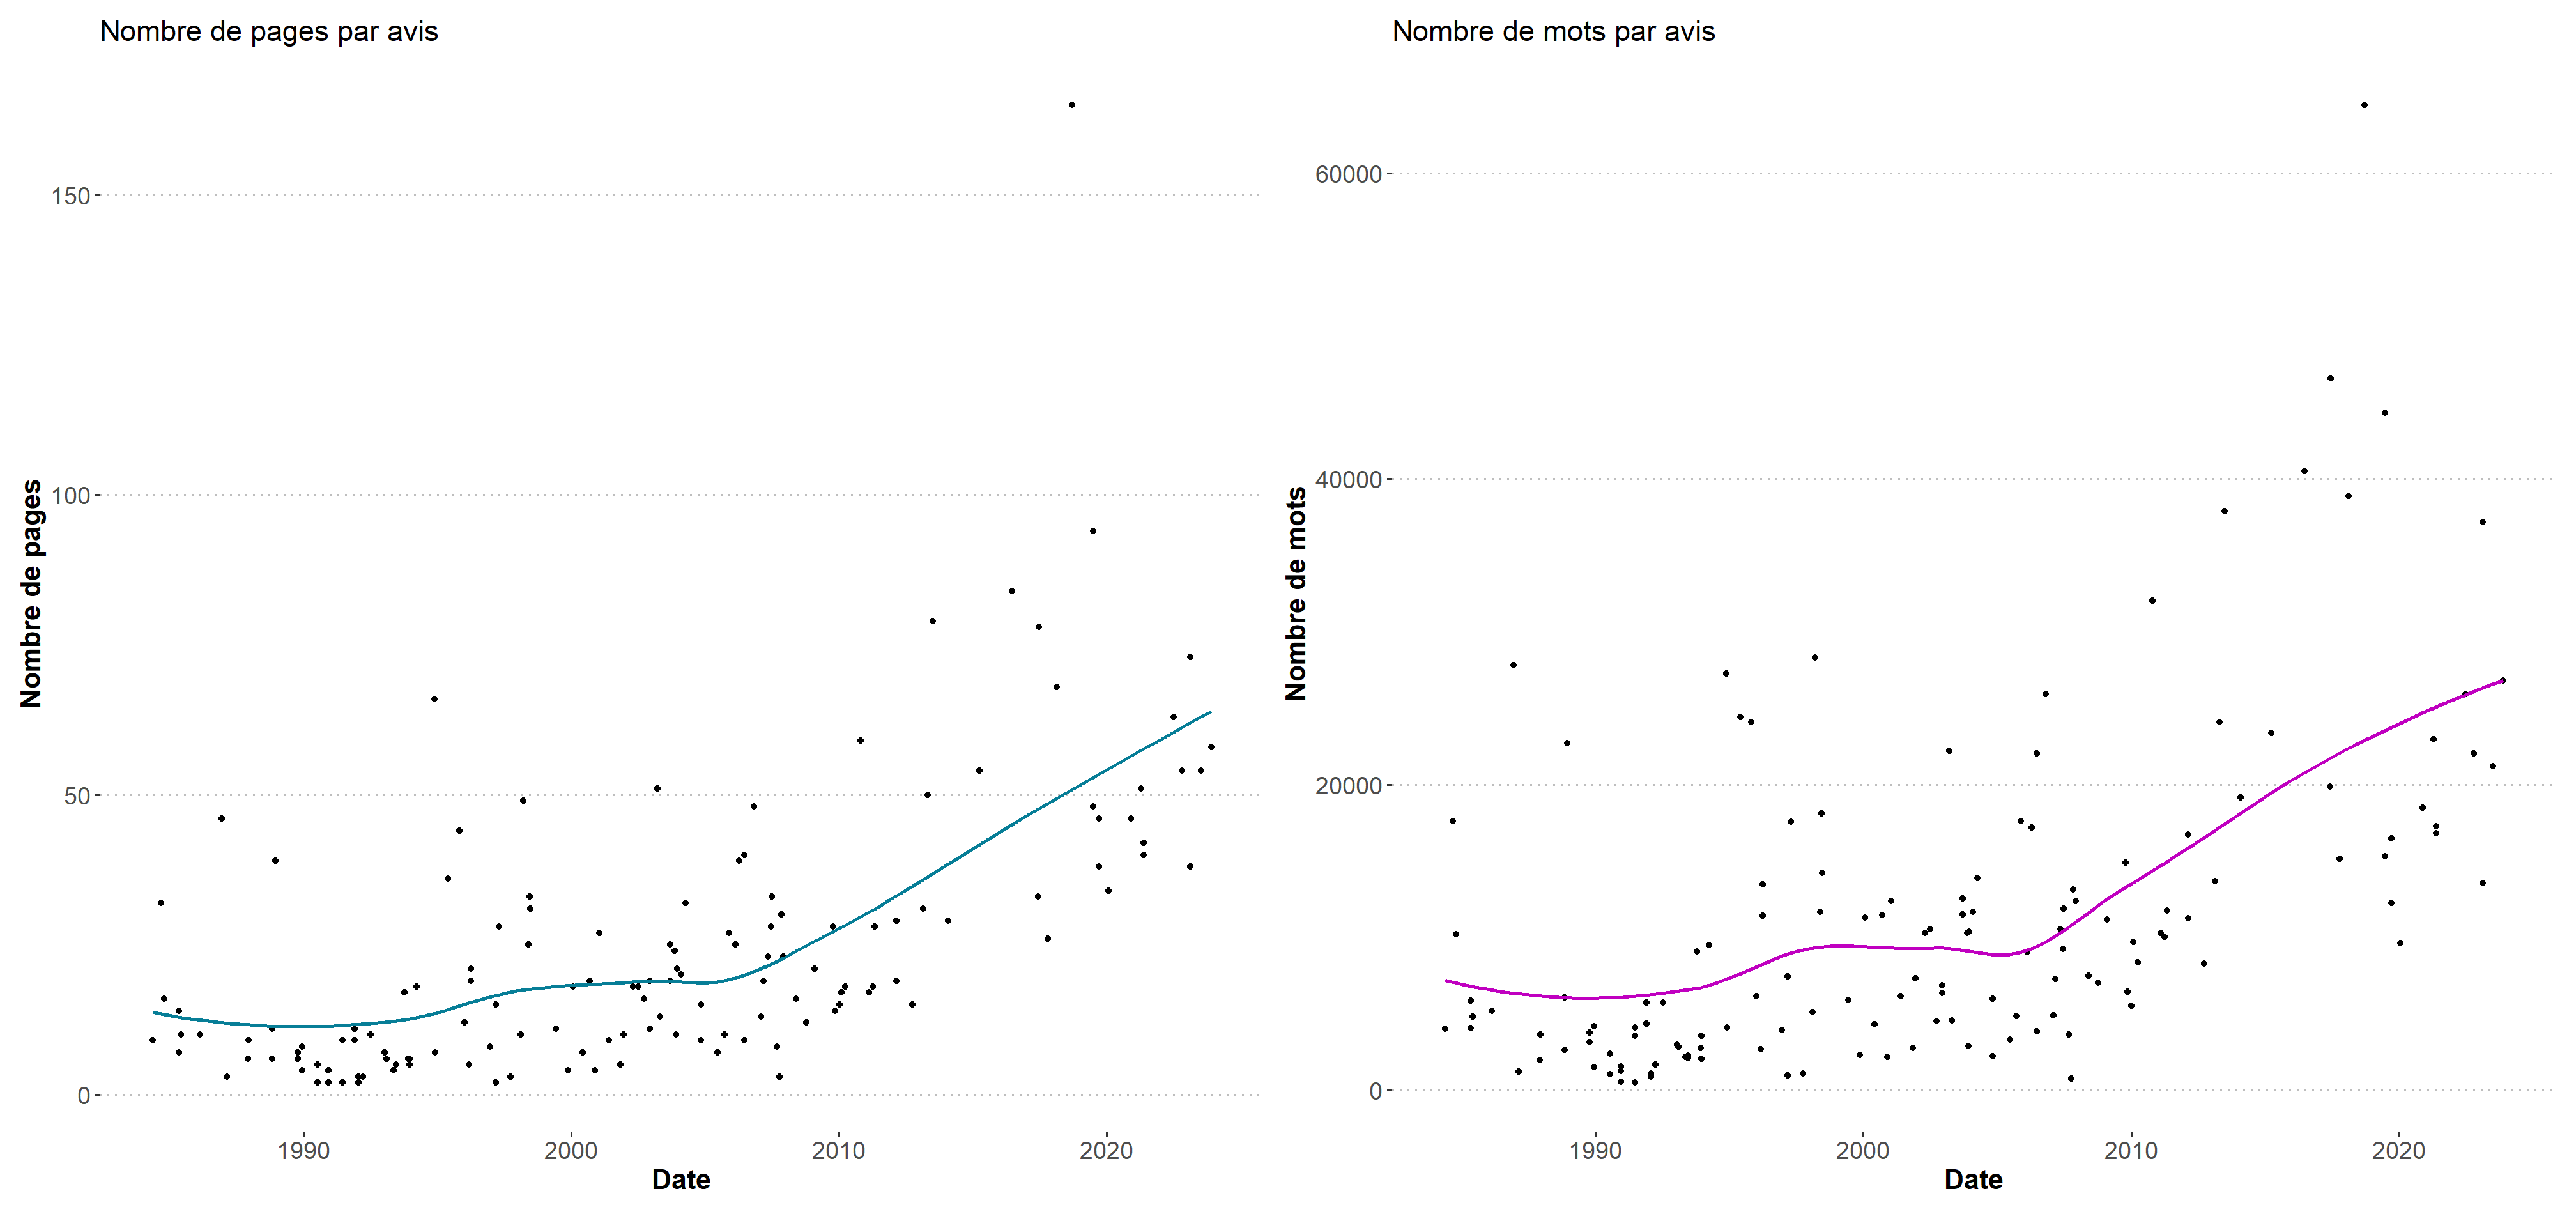
\includegraphics{LDA_report_files/figure-latex/fig-longueur-1.pdf}

}

}

\subcaption{\label{fig-longueur-1}Pages}
\end{minipage}%
%
\begin{minipage}[t]{0.50\linewidth}

{\centering 

\raisebox{-\height}{

\includegraphics{LDA_report_files/figure-latex/fig-longueur-2.pdf}

}

}

\subcaption{\label{fig-longueur-2}Mots}
\end{minipage}%

\caption{\label{fig-longueur}Taille des avis au cours du temps}

\end{figure}

\begin{figure*}

{\centering 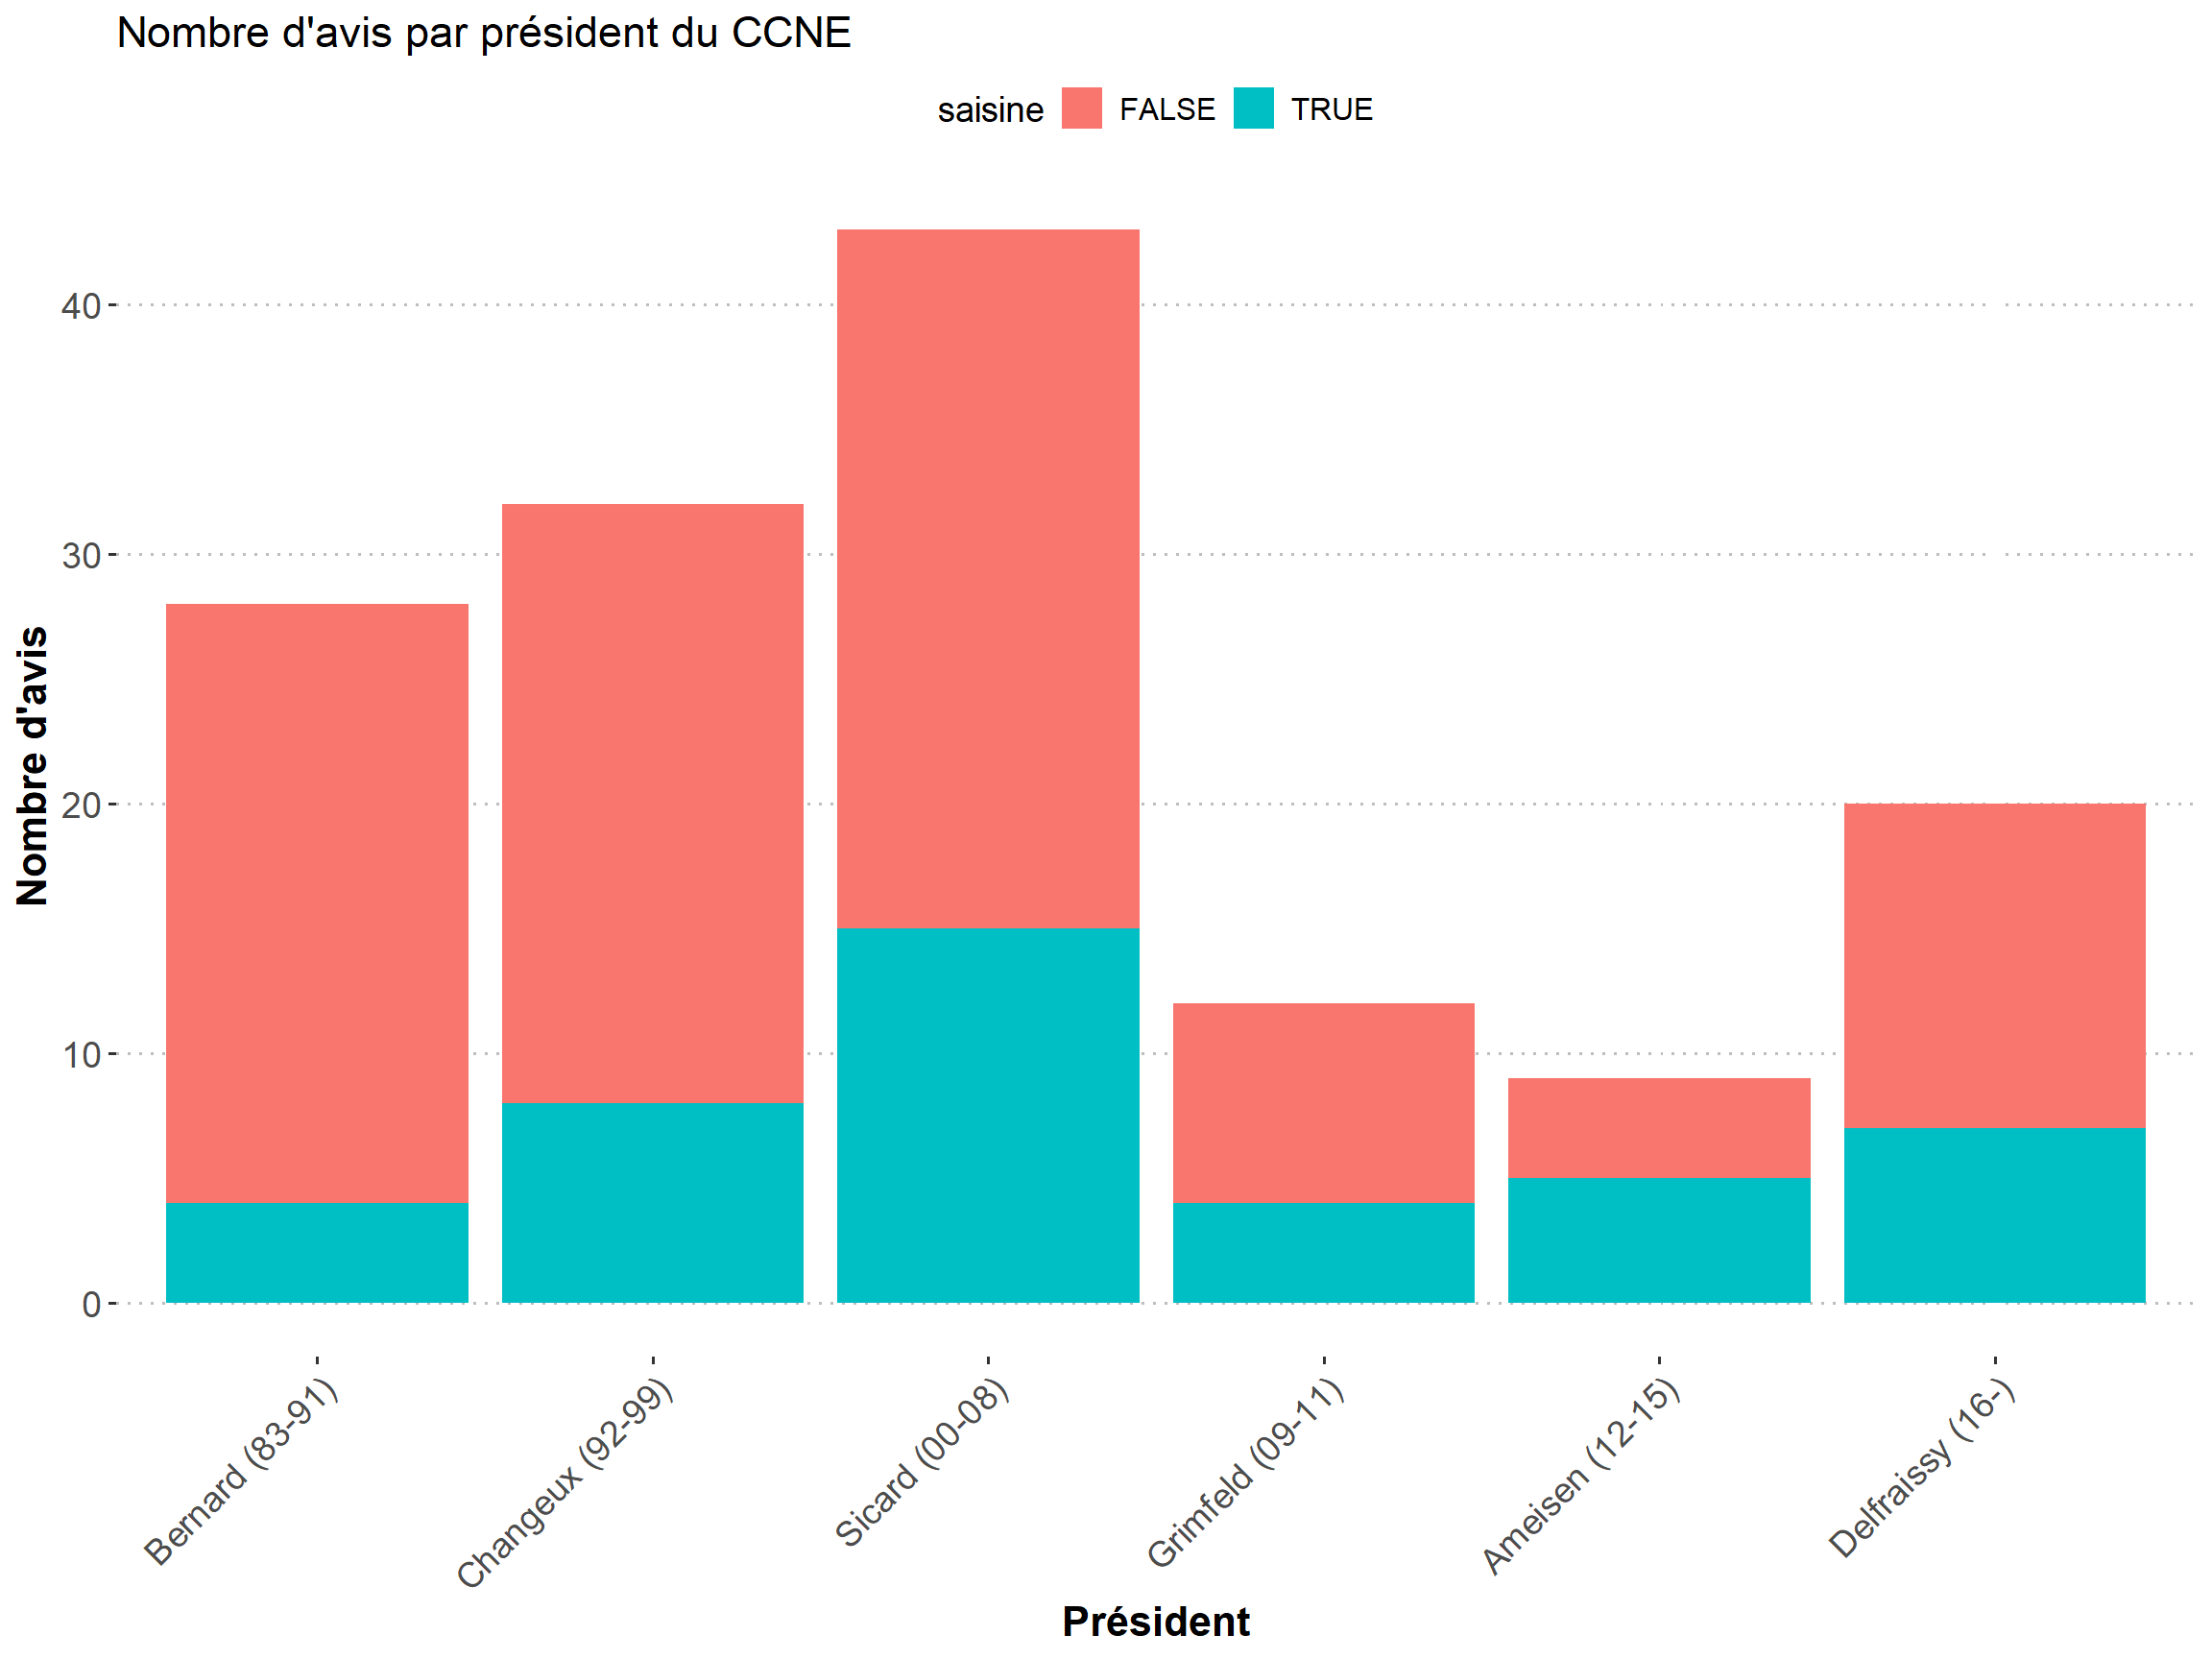
\includegraphics{LDA_report_files/figure-latex/fig-avis_president-1.pdf}

}

\caption{\label{fig-avis_president}Nombre d'avis par président}

\end{figure*}

\begin{figure*}

{\centering \includegraphics{LDA_report_files/figure-latex/fig-avis_president_theme-1.pdf}

}

\caption{\label{fig-avis_president_theme}Thème par président}

\end{figure*}

\hypertarget{preprocessing}{%
\subsection{Preprocessing}\label{preprocessing}}

\hypertarget{contexte-autour-des-mots}{%
\subsubsection{Contexte autour des
mots}\label{contexte-autour-des-mots}}

Pour pouvoir préparer correctement notre tokenisation, il nous faut
regarder le contexte autour de certains mots. Deux exemples importants :
le mot `don' et le mot `personne'.

Le mot don est avant modification des tokens initiaux le mot le plus
fréquent du corpus. Cependant, au regard des 2-grams le suivant présenté
dans la Table~\ref{tbl-contexte_don}, on peut voir que cela désigne
plusieurs objets différents que nous avons rassemblés en quatre
catégories : don de gamètes (d'ovocytes, de spermes etc.), don d'organe,
don de sang, don de cellules. Ce découpage a fait perdre sa place au mot
don.

Un découpage similaire a été opéré pour le mot `personne' : on a
distingué personne handicapée, personne handicapée mentale, personne
malade, personne de confiance, personne agée, personne humaine
potentielle (compromis désignant le foetus) en suivant les résultats de
la Table~\ref{tbl-contexte_personne}

\hypertarget{tbl-contexte_don}{}
\begin{longtable}{rrrrrrrrrrrrrrrrrrrr}
\caption{\label{tbl-contexte_don}Examples de contexte suivant le mot `don' }\tabularnewline

\toprule
du sang & de sang & de gamètes & d ovocytes & de sperme & d organes & d embryons & d ovocyte & d organe & d embryon & à un & entre vivants & à la & d un & et à & a été & contaminant sur & de moelle & d éléments & de leur\\
\midrule
87 & 66 & 55 & 54 & 43 & 36 & 31 & 21 & 18 & 15 & 10 & 10 & 9 & 9 & 8 & 6 & 6 & 6 & 5 & 5\\
\bottomrule
\end{longtable}

\hypertarget{tbl-contexte_personne}{}
\begin{longtable}{rrrrrrrrrrrrrrrrrrrr}
\caption{\label{tbl-contexte_personne}Examples de contexte suivant le mot `personne' }\tabularnewline

\toprule
de confiance & humaine potentielle & handicapée mentale & n est & ne peut & doit être & en fin & et de & atteinte d & en danger & et la & malade ou & malade et & en péril & qui a & dont la & qui est & et le & humaine et & qui en\\
\midrule
84 & 46 & 32 & 24 & 19 & 18 & 17 & 17 & 16 & 14 & 14 & 14 & 13 & 12 & 11 & 9 & 9 & 8 & 8 & 8\\
\bottomrule
\end{longtable}

\begin{table}

\end{table}

\begin{table}

\end{table}

\begin{table}

\end{table}

\begin{table}

\end{table}

\hypertarget{tokenisation-finale}{%
\subsubsection{Tokenisation finale}\label{tokenisation-finale}}

En plus des séparations évoquées plus haut, dans le pré-traitement, on
supprime les dates et nombres présents dans le texte et on regroupe sous
un même dénomination plusieurs ensembles de mots. Par exemple,
l'ensemble `CCNE' ou `comité national consultatif d'éthique' sont
regroupés sous la même domination ou encore, `avortement', `ivg' et
`interruption volontaire de grosse' sont regroupés sous le même token
d'avortement. On supprime aussi un certain nombre de mots dont la
fréquence était élevé mais dont la pertinence semblait être faible
(``peut'', ``comme'' etc.). De plus, en regardant aussi les mots les
plus fréquent on rassemble les pluriels ou les masculins/féminins de
certains adjectifs comme humain/humaine/humains/humaines sous le même
token. Pour finir, on supprime les mots dont il y a moins de 5
occurences dans tout le corpus.

\hypertarget{premiuxe8res-descriptions-du-corpus}{%
\section{Premières descriptions du
corpus}\label{premiuxe8res-descriptions-du-corpus}}

On peut voir sur la Figure~\ref{fig-wordcloud} les mots les plus
fréquents (au moins 750 dans le corpus) représenté sous la forme d'un
wordcloud. On peut voir que malgré le fait d'avoir subdivisé
grossièrement les sens de personne, le terme en lui-même reste le plus
fréquent. Cela tend à confirmer le fait que le CCNE analyse les
problématiques qui lui sont données au regard de la notion de personne
en premier lieu. On retrouve aussi dans ce wordcloud des sujets
essentiels comme le don de gamète, l'enfant, l'embryon, la génétique.

\begin{figure}

{\centering \includegraphics{LDA_report_files/figure-latex/fig-wordcloud-1.pdf}

}

\caption{\label{fig-wordcloud}Mots les plus fréquents dans le corpus. La
taille est proportionnelle à la fréquence.}

\end{figure}

\begin{figure}

{\centering \includegraphics{LDA_report_files/figure-latex/fig-word_time-1.pdf}

}

\caption{\label{fig-word_time}Evolution des mots les plus fréquent du
corpus au cours du temps}

\end{figure}

\hypertarget{analyse-moduxe9lisation-lexicomuxe9trique-par-latent-dirichlet-allocation-et-structural-topic-modelling}{%
\section{Analyse : modélisation lexicométrique par Latent Dirichlet
Allocation et Structural Topic
Modelling}\label{analyse-moduxe9lisation-lexicomuxe9trique-par-latent-dirichlet-allocation-et-structural-topic-modelling}}

\hypertarget{choix-du-nombre-de-topics}{%
\subsection{Choix du nombre de topics}\label{choix-du-nombre-de-topics}}

Pour choisir le nombre de topics de nos modèles, on regarde des
métriques définies par de précédents auteurs (fonction
\texttt{FindTopicsNumber} de \texttt{TopicModels}), présentées sur la
Figure~\ref{fig-lda-metrics}. De plus, on compare pour chaque nombre de
topics la cohérence sémantique et l'exclusivité (fonction
\texttt{searchK} de \texttt{stm}), présenté dans la
Figure~\ref{fig-lda-exclu_cohsem}. L'exclusivité mesure dans quel point
un terme est associé de manière unique à un seul thème, tandis que la
cohérence sémantique évalue le degré de similarité entre les termes au
sein d'un thème, reflétant la cohésion interne et l'interprétabilité du
thème. On voit que le dernier gros gain pour la métrique
\texttt{Deveaud2014} se fait pour onze topics, c'est aussi vers ce
nombre de topics que les autres courbes ont tendance à s'aplatir et donc
qu'augmenter de un le nombre de topics ne donne pas beaucoup plus
d'information tout en rendant plus complexe l'interprétation. On voit
aussi qu'on gagne beaucoup en exclusivité (par rapport à la situation à
8 topics) quand on utilise 11 topics. Chaque topic devrait donc dépendre
sur des mots spécifiques à chacun, même s'il faut renoncer à un peu de
cohérence). Huit topics aurait pu être une bonne alternative.

\begin{verbatim}
NULL
\end{verbatim}

\begin{figure}

{\centering \includegraphics{LDA_report_files/figure-latex/fig-lda-metrics-1.pdf}

}

\caption{\label{fig-lda-metrics}Evolution de différentes métriques en
fonction du nombre de topics}

\end{figure}

\begin{figure}

{\centering \includegraphics{LDA_report_files/figure-latex/fig-lda-exclu_cohsem-1.pdf}

}

\caption{\label{fig-lda-exclu_cohsem}Cohérence sémantique et excluvité
en fonction du nombre de topics}

\end{figure}

\hypertarget{stm-uxe0-onze-topics}{%
\subsection{STM à Onze topics}\label{stm-uxe0-onze-topics}}

On réalise un structural topic modeling avec 11 topics et la formule
suivante :
\texttt{prevalence\ =\textasciitilde{}\ saisine\ +\ divergence\ +\ factor(president)\ +\ factor(theme)\ +\ s(Annee)}.

\hypertarget{description-des-thuxe8mes}{%
\subsubsection{Description des thèmes}\label{description-des-thuxe8mes}}

A partir des mots les plus fréquents - présentés de façon courte dans la
Figure~\ref{fig-stm-summary_prob} et de façon détaillée en annexe dans
la \textbf{?@tbl-stm-full\_prob\_words} - et des mots les plus exclusifs
- de même, résumé figure Figure~\ref{fig-stm-summary_frex}, détails sur
Table~\ref{tbl-stm-full_frex_words}, on peut tenter de donner un premier
sens à nos topics.

En les prenants dans l'ordre de prévalence :

\begin{itemize}
\item
  \textbf{Topic 3:} Correspond probablement au diagnostic génétique et
  prénatal.
\item
  \textbf{Topic 2:} Peut correspondre aux questions de procréation et de
  risques pour l'enfant. L'autisme a malheureusement été traité dans ce
  sens dans un certain nombre d'avis.
\item
  \textbf{Topic 9:} Correspond probablement aux réflexions éthiques
  portant sur la recherche clinique.
\item
  \textbf{Topic 1:} Correspond aux questions relatives aux prélèvements
  de tissus humains.
\item
  \textbf{Topic 6:} Correspond plus spécifiquement aux questions de
  recherche sur l'embryon, comme un sous-cas du topic 1. Il est
  important de rappeler que c'est l'un des thèmes.
\item
  \textbf{Topic 10:} Difficile à distinguer du topic 9, plus
  d'explorations sont nécessaires. On peut penser qu'il est lié aux
  questions de greffes et de transplantations.
\item
  \textbf{Topic 5:} Mélange entre les questions de drogue, de prix des
  médicaments et d'handicaps mentaux. Peut-être un lien commun par
  l'utilisation du vocabulaire de prix ou de travail.
\item
  \textbf{Topic 8:} Semble être un topic sur l'éthique de façon plus
  générale, mais pas forcément sur la recherche clinique. Plutôt sur
  différents problèmes de santé publique : soins, COVID, vaccination,
  autotests comme le montre les plus exclusifs.
\item
  \textbf{Topic 4:} Mélange l'euthanasie et la PMA. C'est possiblement
  lié à un vocabulaire commun autour de l'assistance, comme suggéré dans
  les tableaux détaillés.
\item
  \textbf{Topic 7:} Correspond aux problématiques d'utilisation des
  données médicales avec le mot exclusif `RGPD', par exemple.
\end{itemize}

\begin{Shaded}
\begin{Highlighting}[]
\FunctionTok{plot}\NormalTok{(stm\_lda, }\AttributeTok{type =} \StringTok{"summary"}\NormalTok{, }\AttributeTok{labeltype =} \StringTok{"prob"}\NormalTok{)}
\end{Highlighting}
\end{Shaded}

\begin{figure}

{\centering \includegraphics{LDA_report_files/figure-latex/fig-stm-summary_prob-1.pdf}

}

\caption{\label{fig-stm-summary_prob}Les 3 mots les plus fréquents par
topics. La ligne représente la prévalence dans le corpus du topic.}

\end{figure}

\begin{Shaded}
\begin{Highlighting}[]
\FunctionTok{plot}\NormalTok{(stm\_lda, }\AttributeTok{type =} \StringTok{"summary"}\NormalTok{, }\AttributeTok{labeltype =} \StringTok{"frex"}\NormalTok{)}
\end{Highlighting}
\end{Shaded}

\begin{figure}

{\centering \includegraphics{LDA_report_files/figure-latex/fig-stm-summary_frex-1.pdf}

}

\caption{\label{fig-stm-summary_frex}Les 3 mots les plus exclusifs
(mesure FREX) par topics. La ligne représente la prévalence dans le
corpus du topic.}

\end{figure}

Pour aller plus en détails, on peut regarder les corrélations entre les
topics, présentés dans la Figure~\ref{fig-stm-corr_plot} (et en annexe
la matrice de corrélation complète, Figure~\ref{fig-stm-corr_mat}). On
trouve que seuls les topic 1 et 6 sont très légèrements corrélés, car
ils parlent tous les deux de prélévements chez l'humain. Les autres
topics ne sont pas du tout corrélés entre eux ou voir légèrement
négativement corrélés. Il semble que cela vient de l'initialisation par
les valeurs spectrales.

\begin{figure}

{\centering \includegraphics{LDA_report_files/figure-latex/fig-stm-corr_plot-1.pdf}

}

\caption{\label{fig-stm-corr_plot}STM correlation between topics}

\end{figure}

Pour bien essayer de comprendre les différences entre les topic 9, 10 et
11, on peut les mettre en perspective. On voit que le topic 9 par
rapport au topic 10 est plus orienté recherche scientifique et éthique
tandis que le topic 10 est plus orientés sur des techniques cliniques et
médicales. En faisant une comparaison similaire entre 9 et 11, on voit
que les deux topics parlent d'éthique mais le 9 parle d'éthique de la
recherche scientifique alors qu'on peut penser que le topic 11 se
concentre sur des problématiques particulières (biodiversité, don de
gamète, génétique). Dans cette comparaison, l'opposition entre les mots
personnes et humains nous semblent vraiment intéressante : le traduit
une intention pour le topic 11 surtout sur le corps biologique, tandis
que le topic 9 parle de la personne, donc l'individu dans un sens plus
général.

\begin{figure}

{\centering \includegraphics{LDA_report_files/figure-latex/fig-stm-perspective910-1.pdf}

}

\caption{\label{fig-stm-perspective910}Topic 9 contre Topic 10}

\end{figure}

\begin{figure}

{\centering \includegraphics{LDA_report_files/figure-latex/fig-stm-perspective911-1.pdf}

}

\caption{\label{fig-stm-perspective911}Topic 9 contre Topic 11}

\end{figure}

Pour terminer sur la description des topics, on peut regarder pour
chaque topic, quels avis montrent la plus forte prévalence de topic. On
montre dans la Table~\ref{tbl-stm-top_avis}. Cela permet de nuancer
l'imprétation des topics. On peut ainsi dire que :

\begin{itemize}
\item
  \textbf{Topic 1:} Utilisation de produits issus du corps humain.
\item
  \textbf{Topic 10:} Utilisation de parties du corps humain, incluant la
  greffe et un avis sur l'exposition des corps au musée, soulevé par une
  lettre du Museum d'histoire naturelle.
\item
  \textbf{Topic 11:} Semble recouper plusieurs sujets différents. Peut
  être interprété comme la montée de l'importance de regarder en
  écosystème les questions de santé, y compris la biodiversité et la
  manipulation du génome.
\item
  \textbf{Topic 2:} Correspond à la sexualité, la reproduction et les
  risques, avec des avis sur la contraception et l'enjeu du don du sang
  pour les hommes ayant des rapports avec d'autres hommes.
\item
  \textbf{Topic 3:} Correspond bien au diagnostic prénatal et génétique.
\item
  \textbf{Topic 4:} Semble correspondre à la fin de vie, en incluant la
  santé en prison, en raison d'un grand volet sur la fin de vie en
  prison dans l'avis n°94.
\item
  \textbf{Topic 5:} Correspond à l'usage des drogues et aux risques de
  certains traitements médicamenteux (centoxin, anti-corps autorisé en
  1991, puis retiré en 1993 en raison de falsifications). Interprétable
  comme substances et risques.
\item
  \textbf{Topic 6:} Correspond au thème de l'embryon.
\item
  \textbf{Topic 7:} Thème des données de santé.
\item
  \textbf{Topic 8:} Éthique en situation de santé publique, incluant les
  pandémies, les vaccinations et la santé des migrants.
\item
  \textbf{Topic 9:} Éthique et recherche, notamment l'étonnant avis
  n°131 dédié aux expérimentations en sciences de l'éducation, sciences
  cognitives et psychologie, expliquant la prévalence du terme
  ``pédagogie''.
\end{itemize}

\hypertarget{tbl-stm-top_avis}{}
\begin{table}
\caption{\label{tbl-stm-top_avis}Top 3 des avis avec le plus grande prévalence par topic }\tabularnewline

\centering
\begin{tabular}{r|l|l|l|l|r}
\hline
N°avis & Titre & Date & President & Topic & Prevalence\\
\hline
117 & Utilisation des cellules souches issues du sang de cordon ombilical, du cordon lui-même et du placenta et leur conservation en biobanques. Questionnement éthique. & 2012-02-23 & Ameisen (12-15) & Topic1 & 0.999\\
\hline
28 & Avis sur la transfusion sanguine au regard de la non-commercialisation du corps humain. Rapport. & 1991-12-02 & Bernard (83-91) & Topic1 & 0.999\\
\hline
16 & Avis sur les greffes de cellules nerveuses dans le traitement de la maladie de Parkinson. Rapport. & 1989-10-16 & Bernard (83-91) & Topic1 & 0.999\\
\hline
82 & L'allotransplantation de tissu composite (ATC) au niveau de la face (Greffe totale ou partiale d'un visage) & 2004-02-06 & Sicard (00-08) & Topic10 & 0.999\\
\hline
111 & Avis sur les problèmes éthiques posés par l’utilisation des cadavres à des fins de conservation ou d’exposition muséale & 2010-01-07 & Grimfeld (09-11) & Topic10 & 0.995\\
\hline
12 & Avis sur l'expérimentation médicale et scientifque sur des sujets en état de mort cérébrale. Rapport. & 1988-11-07 & Bernard (83-91) & Topic10 & 0.995\\
\hline
125 & Biodiversité et santé : nouvelles relations entre l’humanité et le vivant & 2017-06-07 & Delfraissy (16-) & Topic11 & 0.999\\
\hline
134 & L’adoption : accroître la transparence des procédures pour favoriser l’objectivité et la qualité des choix & 2020-01-23 & Delfraissy (16-) & Topic11 & 0.989\\
\hline
133 & Enjeux éthiques des modifications ciblées du génome : entre espoir et vigilance & 2019-09-19 & Delfraissy (16-) & Topic11 & 0.924\\
\hline
123 & Questionnement éthique et observations concernant la contre-indication permanente du don de sang pour tout homme déclarant avoir eu une ou des relation(s) sexuelle(s) avec un ou plusieurs homme(s) & 2015-03-28 & Ameisen (12-15) & Topic2 & 1.000\\
\hline
49 & Avis sur la contraception chez les personnes handicapées mentales. Rapport & 1996-04-03 & Changeux (92-99) & Topic2 & 0.993\\
\hline
50 & Rapport sur la stérilisation envisagée comme mode de contraception définitive. & 1996-04-03 & Changeux (92-99) & Topic2 & 0.956\\
\hline
46 & Avis et recommandations sur "Génétique et médecine: de la prédiction à la prévention". Rapport. & 1995-10-30 & Changeux (92-99) & Topic3 & 1.000\\
\hline
120 & Questions éthiques associées au développement des tests génétiques fœtaux sur sang maternel & 2013-04-25 & Ameisen (12-15) & Topic3 & 0.999\\
\hline
5 & Avis sur les problèmes posés par le diagnostic prénatal et périnatal. Rapport. & 1985-05-13 & Bernard (83-91) & Topic3 & 0.999\\
\hline
121 & Fin de vie, autonomie de la personne, volonté de mourir & 2013-06-30 & Ameisen (12-15) & Topic4 & 1.000\\
\hline
139 & Questions éthiques relatives aux situations de fin de vie : autonomie et solidarité & 2022-06-30 & Delfraissy (16-) & Topic4 & 1.000\\
\hline
94 & La santé et la médecine en prison & 2006-10-26 & Sicard (00-08) & Topic4 & 0.999\\
\hline
43 & Rapports du Comité consultatif national d'éthique pour les sciences de la vie et de la santé sur les toxicomanies. & 1994-11-23 & Changeux (92-99) & Topic5 & 1.000\\
\hline
32 & Avis sur l'opportunité et le type d'essai à mettre en oeuvre pour préciser les indications du centoxin. Rapport. & 1992-07-10 & Changeux (92-99) & Topic5 & 0.999\\
\hline
34 & Avis sur l'utilisation de placebo dans les essais thérapeutiques d'antidépresseurs. Rapport. & 1993-02-09 & Changeux (92-99) & Topic5 & 0.999\\
\hline
112 & Une réflexion éthique sur la recherche sur les cellules d’origine embryonnaire humaine, et la recherche sur l’embryon humain in vitro & 2010-10-21 & Grimfeld (09-11) & Topic6 & 1.000\\
\hline
54 & Réponse au Président de la République au sujet du clonage reproductif. & 1997-04-22 & Changeux (92-99) & Topic6 & 0.999\\
\hline
67 & Avis sur l'avant-projet de révision des lois de bioéthique & 2001-01-18 & Sicard (00-08) & Topic6 & 0.999\\
\hline
143 & Plateformes de données de santé & 2023-02-16 & Delfraissy (16-) & Topic7 & 1.000\\
\hline
130 & Données massives et santé : Etat des lieux, prospective et nouvelles questions éthiques & 2019-06-29 & Delfraissy (16-) & Topic7 & 1.000\\
\hline
141 & Diagnostic Médical et Intelligence Artificielle : Enjeux Ethiques & 2023-11-24 & Delfraissy (16-) & Topic7 & 1.000\\
\hline
144 & La vaccination des professionnels exerçant dans les secteurs sanitaires et médico-sociaux : Sécurité des patients, responsabilité des professionnels et contexte social & 2023-07-06 & Delfraissy (16-) & Topic8 & 1.000\\
\hline
106 & Questions éthiques soulevées par une possible pandémie grippale & 2009-02-05 & Grimfeld (09-11) & Topic8 & 0.999\\
\hline
127 & santé des migrants et exigence éthique & 2017-10-16 & Delfraissy (16-) & Topic8 & 0.955\\
\hline
45 & Avis sur les questions éthiques posées par la transmission de l'information scientifique relative à la recherche biologique et médicale. Rapport. & 1995-05-31 & Changeux (92-99) & Topic9 & 1.000\\
\hline
131 & Cadre éthique de l’expérimentation pédagogique en situation réelle & 2019-06-27 & Delfraissy (16-) & Topic9 & 0.998\\
\hline
29 & Avis relatif aux Comités d'éthique & 1992-01-27 & Changeux (92-99) & Topic9 & 0.998\\
\hline
\end{tabular}
\end{table}

On obtient finalement les interprésentations grossières présentés dans
Table~\ref{tbl-stm-interpretations}.

\hypertarget{tbl-stm-interpretations}{}
\begin{table}
\caption{\label{tbl-stm-interpretations}Interprétations de nos topics }\tabularnewline

\centering
\begin{tabular}{r|l}
\hline
N° Avis & Interprétation\\
\hline
1 & Produits corpus humains\\
\hline
2 & Rapports sexuels et risques\\
\hline
3 & Diagnostic génétique\\
\hline
4 & Fin de vie et assistance\\
\hline
5 & Substances et risques\\
\hline
6 & Embryon\\
\hline
7 & Données\\
\hline
8 & Santé publique\\
\hline
9 & Recherche\\
\hline
10 & Corps\\
\hline
11 & Ecosystèmes ?\\
\hline
\end{tabular}
\end{table}

\hypertarget{effets-des-muxe9tadonnuxe9es-sur-la-pruxe9valence}{%
\subsubsection{Effets des métadonnées sur la
prévalence}\label{effets-des-muxe9tadonnuxe9es-sur-la-pruxe9valence}}

Grâce à notre modélisation par un structural topic modelling, on peut
regarder l'effet de nos métadata sur la prévalence des thèmes.
Globalement dans les tableaux présentés
Table~\ref{tbl-stm-main_effects}, il y a une certaines cohérences entre
notre interprétation et l'effet des covariables:

\begin{itemize}
\item
  \textbf{Topic 1:} Utilisation du corps humain

  \begin{itemize}
  \tightlist
  \item
    Croît avec la thématique greffe, ce qui est logique vu qu'il semble
    parler d'utiliser les tissus humains.
  \item
    Intéressant de noter que c'est un sujet qui décroît avec tous les
    présidents depuis 1992.
  \end{itemize}
\item
  \textbf{Topic 2:} Effets positifs et significatifs

  \begin{itemize}
  \tightlist
  \item
    Respectivement à 1\% et à 10\% pour les thèmes sexualité, genre, et
    du thème procréation.
  \item
    Logique pour le topic associé aux risques de ces pratiques (?).
  \end{itemize}
\item
  \textbf{Topic 3:} Topic extrêmement transversal aux questionnements du
  CCNE.
\item
  \textbf{Topic 4:} Effet très très fortement significatif du thème fin
  de vie, confirmant notre interprétation.
\item
  \textbf{Topics 5, 6, et 11:} Effets et interprétations complexes à
  mettre en lien.
\item
  \textbf{Topics 7 et 8:} Influence des questions de santé publique,
  logique avec nos interprétations.
\item
  \textbf{Topic 9:} Significativité des politiques de santé et de la
  recherche.
\item
  \textbf{Topic 10:} Influence du corps (thème des greffes), mais
  surtout l'importance du droit.
\end{itemize}

Pour l'interprétation des autres covariables, on peut noter quelques
points intéressants. L'actuel président (depuis 2016) Jean-François
Delfraissy semble marquer quelques ruptures : il a un effet positif et
significatif sur les topics 7, 8, et 11 qui marquent un tournant vers la
santé publique et les écosystèmes et non plus simplement une éthique de
la pratique clinique. Cela semble aller dans le sens que le CCNE s'est
ouvert à insérer sa réflexion dans la société et la nature.

Une autre rupture notable est le topic 11 où tous les présidents du CCNE
depuis 1992 ont un effet négatif (et significatif à 5\%) sur sa
prévalence. Mais cela semble difficile de le faire correspondre avec un
événement historique ou un changement structurel du CCNE. De même pour
le topic 5 concernant les risques des médicaments qui semblent avoir été
sous évoqué durant la présidence de Jean Claude Aimensen de 2012 à 2015.

L'essentiel des autres topics sont guidés principalement par leurs
sujets et thèmes ce qui laisse à penser une cohérence de vocabulaire et
lexicographique au cours du temps.

Dernière remarque, contrairement à ce qu'on pourrait penser, il n'y a
peu d'effet sur les thèmes abordés du fait d'avoir été saisi par une
institution officielle. La demande politique semble faire baisser (de
façon significatif à 10\%) la prévalence du topic 2 ``sexualité et
risque'' et du topic 10 ``corps''. Si dans le second cas, cela semble
relativement logique car ce sont des préocupations de terrains (de
chirurgiens ou de musées), le premier cas semble d'intérêt publique
surtout avec la crise du SIDA. Une explication possible pour ce résultat
étonnant est que la crise du VIH fait l'objet de ses propres
négociations et réflexions en dehors du CCNE.

\hypertarget{tbl-stm-main_effects}{}
\begin{table}
\caption{\label{tbl-stm-main_effects}Effets significatifs des métadonnées sur les différents topics }\tabularnewline

\centering
\begin{tabular}{}
\hline

\hline
\end{tabular}
\end{table}

\begin{table}

\caption{Effets structurels significatifs sur la prévalence des thèmes pour le topic 1 Produits corpus humains 
}
\centering
\begin{tabular}[t]{l|r|r|r|r|l}
\hline
  & Estimate & Std. Error & t value & Pr(>|t|) & signif\\
\hline
(Intercept) & 0.278 & 0.122 & 2.290 & 0.024 & ••\\
\hline
factor(president)Changeux (92-99) & -0.200 & 0.081 & -2.468 & 0.015 & ••\\
\hline
factor(president)Sicard (00-08) & -0.224 & 0.083 & -2.691 & 0.008 & •••\\
\hline
factor(president)Grimfeld (09-11) & -0.258 & 0.099 & -2.594 & 0.011 & ••\\
\hline
factor(president)Delfraissy (16-) & -0.272 & 0.091 & -2.999 & 0.003 & •••\\
\hline
\multicolumn{6}{l}{\rule{0pt}{1em}\textit{Note: }}\\
\multicolumn{6}{l}{\rule{0pt}{1em}Signif. codes, p<t : 0.001 ‘····’ 0.01 ‘···’ 0.05 ‘··’ 0.1 ‘·’ }\\
\end{tabular}
\end{table}

\begin{table}

\caption{Effets structurels significatifs sur la prévalence des thèmes pour le topic 2 Rapports sexuels et risques 
}
\centering
\begin{tabular}[t]{l|r|r|r|r|l}
\hline
  & Estimate & Std. Error & t value & Pr(>|t|) & signif\\
\hline
factor(theme)Sexualité, Genre & 0.511 & 0.204 & 2.509 & 0.013 & ••\\
\hline
\multicolumn{6}{l}{\rule{0pt}{1em}\textit{Note: }}\\
\multicolumn{6}{l}{\rule{0pt}{1em}Signif. codes, p<t : 0.001 ‘····’ 0.01 ‘···’ 0.05 ‘··’ 0.1 ‘·’ }\\
\end{tabular}
\end{table}

\begin{table}

\caption{Effets structurels significatifs sur la prévalence des thèmes pour le topic 3 Diagnostic génétique 
}
\centering
\begin{tabular}[t]{l|r|r|r|r|l}
\hline
  & Estimate & Std. Error & t value & Pr(>|t|) & signif\\
\hline
(Intercept) & 0.304 & 0.146 & 2.078 & 0.040 & ••\\
\hline
factor(theme)Conditions de vie & -0.327 & 0.148 & -2.210 & 0.029 & ••\\
\hline
factor(theme)Début de la vie & -0.295 & 0.152 & -1.950 & 0.054 & ••\\
\hline
factor(theme)Don, consentement & -0.293 & 0.152 & -1.929 & 0.056 & ••\\
\hline
factor(theme)Neurosciences, comportements & -0.281 & 0.163 & -1.724 & 0.087 & ••\\
\hline
factor(theme)Politiques de santé & -0.260 & 0.155 & -1.673 & 0.097 & ••\\
\hline
factor(theme)Recherche & -0.346 & 0.160 & -2.166 & 0.032 & ••\\
\hline
factor(theme)Sexualité, Genre & -0.374 & 0.166 & -2.252 & 0.026 & ••\\
\hline
factor(theme)Société & -0.335 & 0.160 & -2.091 & 0.039 & ••\\
\hline
factor(theme)Viellissement, fin de vie & -0.300 & 0.155 & -1.935 & 0.055 & ••\\
\hline
\multicolumn{6}{l}{\rule{0pt}{1em}\textit{Note: }}\\
\multicolumn{6}{l}{\rule{0pt}{1em}Signif. codes, p<t : 0.001 ‘····’ 0.01 ‘···’ 0.05 ‘··’ 0.1 ‘·’ }\\
\end{tabular}
\end{table}

\begin{table}

\caption{Effets structurels significatifs sur la prévalence des thèmes pour le topic 4 Fin de vie et assistance 
}
\centering
\begin{tabular}[t]{l|r|r|r|r|l}
\hline
  & Estimate & Std. Error & t value & Pr(>|t|) & signif\\
\hline
factor(theme)Don, consentement & 0.234 & 0.114 & 2.046 & 0.043 & ••\\
\hline
factor(theme)Viellissement, fin de vie & 0.636 & 0.132 & 4.803 & 0.000 & ••••\\
\hline
\multicolumn{6}{l}{\rule{0pt}{1em}\textit{Note: }}\\
\multicolumn{6}{l}{\rule{0pt}{1em}Signif. codes, p<t : 0.001 ‘····’ 0.01 ‘···’ 0.05 ‘··’ 0.1 ‘·’ }\\
\end{tabular}
\end{table}

\begin{table}

\caption{Effets structurels significatifs sur la prévalence des thèmes pour le topic 5 Substances et risques 
}
\centering
\begin{tabular}[t]{l|r|r|r|r|l}
\hline
  & Estimate & Std. Error & t value & Pr(>|t|) & signif\\
\hline
factor(president)Changeux (92-99) & 0.136 & 0.072 & 1.884 & 0.062 & ••\\
\hline
factor(president)Ameisen (12-15) & -0.170 & 0.101 & -1.683 & 0.095 & ••\\
\hline
factor(theme)Neurosciences, comportements & 0.271 & 0.147 & 1.842 & 0.068 & ••\\
\hline
\multicolumn{6}{l}{\rule{0pt}{1em}\textit{Note: }}\\
\multicolumn{6}{l}{\rule{0pt}{1em}Signif. codes, p<t : 0.001 ‘····’ 0.01 ‘···’ 0.05 ‘··’ 0.1 ‘·’ }\\
\end{tabular}
\end{table}

\begin{table}

\caption{Effets structurels significatifs sur la prévalence des thèmes pour le topic 6 Embryon 
}
\centering
\begin{tabular}[t]{l|r|r|r|r|l}
\hline
  & Estimate & Std. Error & t value & Pr(>|t|) & signif\\
\hline
factor(theme)Début de la vie & 0.262 & 0.155 & 1.685 & 0.095 & ••\\
\hline
\multicolumn{6}{l}{\rule{0pt}{1em}\textit{Note: }}\\
\multicolumn{6}{l}{\rule{0pt}{1em}Signif. codes, p<t : 0.001 ‘····’ 0.01 ‘···’ 0.05 ‘··’ 0.1 ‘·’ }\\
\end{tabular}
\end{table}

\begin{table}

\caption{Effets structurels significatifs sur la prévalence des thèmes pour le topic 7 Données 
}
\centering
\begin{tabular}[t]{l|r|r|r|r|l}
\hline
  & Estimate & Std. Error & t value & Pr(>|t|) & signif\\
\hline
factor(president)Delfraissy (16-) & 0.114 & 0.051 & 2.239 & 0.027 & ••\\
\hline
factor(theme)Santé et bien-être & 0.912 & 0.131 & 6.937 & 0.000 & ••••\\
\hline
factor(theme)Société & 0.543 & 0.110 & 4.940 & 0.000 & ••••\\
\hline
\multicolumn{6}{l}{\rule{0pt}{1em}\textit{Note: }}\\
\multicolumn{6}{l}{\rule{0pt}{1em}Signif. codes, p<t : 0.001 ‘····’ 0.01 ‘···’ 0.05 ‘··’ 0.1 ‘·’ }\\
\end{tabular}
\end{table}

\begin{table}

\caption{Effets structurels significatifs sur la prévalence des thèmes pour le topic 8 Santé publique 
}
\centering
\begin{tabular}[t]{l|r|r|r|r|l}
\hline
  & Estimate & Std. Error & t value & Pr(>|t|) & signif\\
\hline
factor(president)Delfraissy (16-) & 0.173 & 0.080 & 2.171 & 0.032 & ••\\
\hline
factor(theme)Greffes, vaccin & 0.352 & 0.154 & 2.290 & 0.024 & ••\\
\hline
factor(theme)Politiques de santé & 0.290 & 0.140 & 2.064 & 0.041 & ••\\
\hline
factor(theme)Professions de santé & 0.307 & 0.174 & 1.761 & 0.081 & ••\\
\hline
factor(theme)Viellissement, fin de vie & 0.236 & 0.130 & 1.811 & 0.073 & ••\\
\hline
\multicolumn{6}{l}{\rule{0pt}{1em}\textit{Note: }}\\
\multicolumn{6}{l}{\rule{0pt}{1em}Signif. codes, p<t : 0.001 ‘····’ 0.01 ‘···’ 0.05 ‘··’ 0.1 ‘·’ }\\
\end{tabular}
\end{table}

\begin{table}

\caption{Effets structurels significatifs sur la prévalence des thèmes pour le topic 9 Recherche 
}
\centering
\begin{tabular}[t]{l|r|r|r|r|l}
\hline
  & Estimate & Std. Error & t value & Pr(>|t|) & signif\\
\hline
factor(theme)Politiques de santé & 0.413 & 0.149 & 2.780 & 0.006 & •••\\
\hline
factor(theme)Recherche & 0.320 & 0.156 & 2.056 & 0.042 & ••\\
\hline
\multicolumn{6}{l}{\rule{0pt}{1em}\textit{Note: }}\\
\multicolumn{6}{l}{\rule{0pt}{1em}Signif. codes, p<t : 0.001 ‘····’ 0.01 ‘···’ 0.05 ‘··’ 0.1 ‘·’ }\\
\end{tabular}
\end{table}

\begin{table}

\caption{Effets structurels significatifs sur la prévalence des thèmes pour le topic 10 Corps 
}
\centering
\begin{tabular}[t]{l|r|r|r|r|l}
\hline
  & Estimate & Std. Error & t value & Pr(>|t|) & signif\\
\hline
saisineTRUE & -0.088 & 0.049 & -1.802 & 0.074 & ••\\
\hline
factor(theme)Don, consentement & 0.256 & 0.117 & 2.179 & 0.031 & ••\\
\hline
factor(theme)Greffes, vaccin & 0.306 & 0.139 & 2.200 & 0.030 & ••\\
\hline
factor(theme)Législation, droits & 0.346 & 0.123 & 2.813 & 0.006 & •••\\
\hline
\multicolumn{6}{l}{\rule{0pt}{1em}\textit{Note: }}\\
\multicolumn{6}{l}{\rule{0pt}{1em}Signif. codes, p<t : 0.001 ‘····’ 0.01 ‘···’ 0.05 ‘··’ 0.1 ‘·’ }\\
\end{tabular}
\end{table}

\begin{table}

\caption{Effets structurels significatifs sur la prévalence des thèmes pour le topic 11 Ecosystèmes ? 
}
\centering
\begin{tabular}[t]{l|r|r|r|r|l}
\hline
  & Estimate & Std. Error & t value & Pr(>|t|) & signif\\
\hline
factor(president)Delfraissy (16-) & 0.201 & 0.070 & 2.857 & 0.005 & •••\\
\hline
factor(theme)Parentalité, filiation & 0.313 & 0.154 & 2.029 & 0.045 & ••\\
\hline
\multicolumn{6}{l}{\rule{0pt}{1em}\textit{Note: }}\\
\multicolumn{6}{l}{\rule{0pt}{1em}Signif. codes, p<t : 0.001 ‘····’ 0.01 ‘···’ 0.05 ‘··’ 0.1 ‘·’ }\\
\end{tabular}
\end{table}

\begin{figure}

{\centering \includegraphics{LDA_report_files/figure-latex/fig-stm-time-1.pdf}

}

\caption{\label{fig-stm-time}Prevalence des topics au cours du temps
dans les documents (présentant une prévalence d'au moins 0.1)}

\end{figure}

\hypertarget{annexe}{%
\section{Annexe}\label{annexe}}

\hypertarget{stm-uxe0-11-topics}{%
\subsection{STM à 11 topics}\label{stm-uxe0-11-topics}}

\hypertarget{labelisation-des-topics}{%
\subsubsection{Labelisation des topics}\label{labelisation-des-topics}}

\includegraphics{LDA_report_files/figure-latex/unnamed-chunk-36-1.pdf}

\begin{table}
\caption{Ensemble des 15 mots les plus fréquents par topic}\tabularnewline

\centering
\begin{tabular}{}
\hline

\hline
\end{tabular}
\end{table}

\includegraphics{LDA_report_files/figure-latex/tbl-stm-full_frex_words-1.pdf}

\hypertarget{tbl-stm-full_frex_words}{}
\begin{table}
\caption{\label{tbl-stm-full_frex_words}Ensemble des 15 mots les plus exclusifs par topic }\tabularnewline

\centering
\begin{tabular}{}
\hline

\hline
\end{tabular}
\end{table}

\hypertarget{liens-entre-les-topics}{%
\subsubsection{Liens entre les topics}\label{liens-entre-les-topics}}

\begin{figure}

{\centering \includegraphics{LDA_report_files/figure-latex/fig-stm-corr_mat-1.pdf}

}

\caption{\label{fig-stm-corr_mat}Matrice de corrélation entre les
topics}

\end{figure}

\hypertarget{tables-compluxe8tes-des-effets-structurelles}{%
\subsubsection{Tables complètes des effets
structurelles}\label{tables-compluxe8tes-des-effets-structurelles}}

\begin{table}

\caption{\label{tbl-stm-full_reg_tab}Effets des métadonnées sur les
différents topics}\begin{minipage}[t]{\linewidth}
\subcaption{\label{tbl-stm-full_reg_tab-1}Effets structurels sur la prévalence des thèmes pour le topic 1 1 Produits corpus humains}

{\centering 

\centering
\begin{tabular}[t]{l|r|r|r|r|l}
\hline
  & Estimate & Std. Error & t value & Pr(>|t|) & signif\\
\hline
(Intercept) & 0.085 & 0.187 & 0.454 & 0.650 & \\
\hline
saisineTRUE & -0.075 & 0.054 & -1.390 & 0.168 & ••\\
\hline
divergenceTRUE & 0.006 & 0.114 & 0.049 & 0.961 & \\
\hline
factor(president)Changeux (92-99) & -0.280 & 0.250 & -1.119 & 0.265 & ••\\
\hline
factor(president)Sicard (00-08) & -0.221 & 0.357 & -0.619 & 0.537 & \\
\hline
factor(president)Grimfeld (09-11) & -0.108 & 0.497 & -0.218 & 0.828 & \\
\hline
factor(president)Ameisen (12-15) & 0.314 & 0.567 & 0.555 & 0.580 & \\
\hline
factor(president)Delfraissy (16-) & 0.289 & 0.634 & 0.455 & 0.650 & \\
\hline
factor(theme)Autres maladies & 0.152 & 0.132 & 1.150 & 0.253 & ••\\
\hline
factor(theme)Conditions de vie & 0.033 & 0.132 & 0.250 & 0.803 & \\
\hline
factor(theme)Début de la vie & 0.081 & 0.136 & 0.597 & 0.552 & \\
\hline
factor(theme)Don, consentement & 0.246 & 0.135 & 1.822 & 0.071 & ••\\
\hline
factor(theme)Génétique et Diagnostic & -0.101 & 0.134 & -0.748 & 0.456 & ••\\
\hline
factor(theme)Greffes, vaccin & 0.343 & 0.164 & 2.091 & 0.039 & ••\\
\hline
factor(theme)Législation, droits & 0.115 & 0.143 & 0.803 & 0.424 & ••\\
\hline
factor(theme)Lois de bioéthique & 0.114 & 0.235 & 0.484 & 0.629 & \\
\hline
factor(theme)Maladies génétiques et thérapies & 0.058 & 0.131 & 0.444 & 0.658 & \\
\hline
factor(theme)Neurosciences, comportements & -0.070 & 0.135 & -0.515 & 0.607 & \\
\hline
factor(theme)Parentalité, filiation & -0.020 & 0.196 & -0.100 & 0.920 & \\
\hline
factor(theme)Politiques de santé & -0.046 & 0.132 & -0.348 & 0.728 & \\
\hline
factor(theme)Procréation & 0.012 & 0.152 & 0.078 & 0.938 & \\
\hline
factor(theme)Professions de santé & 0.032 & 0.174 & 0.181 & 0.857 & \\
\hline
factor(theme)Recherche & 0.021 & 0.137 & 0.156 & 0.877 & \\
\hline
factor(theme)Santé et bien-être & 0.233 & 0.289 & 0.808 & 0.421 & ••\\
\hline
factor(theme)Sexualité, Genre & -0.038 & 0.154 & -0.247 & 0.806 & \\
\hline
factor(theme)Société & 0.074 & 0.149 & 0.497 & 0.620 & \\
\hline
factor(theme)Viellissement, fin de vie & -0.096 & 0.134 & -0.717 & 0.475 & ••\\
\hline
s(Annee)1 & -0.192 & 0.376 & -0.511 & 0.611 & \\
\hline
s(Annee)2 & 0.462 & 0.284 & 1.626 & 0.107 & ••\\
\hline
s(Annee)3 & 0.136 & 0.421 & 0.323 & 0.748 & \\
\hline
s(Annee)4 & 0.325 & 0.305 & 1.064 & 0.290 & ••\\
\hline
s(Annee)5 & 0.160 & 0.498 & 0.321 & 0.749 & \\
\hline
s(Annee)6 & 0.106 & 0.391 & 0.272 & 0.786 & \\
\hline
s(Annee)7 & 0.101 & 0.670 & 0.151 & 0.880 & \\
\hline
s(Annee)8 & -0.665 & 0.692 & -0.961 & 0.339 & ••\\
\hline
s(Annee)9 & -0.174 & 0.723 & -0.241 & 0.810 & \\
\hline
s(Annee)10 & -0.536 & 0.647 & -0.829 & 0.409 & ••\\
\hline
\multicolumn{6}{l}{\rule{0pt}{1em}\textit{Note: }}\\
\multicolumn{6}{l}{\rule{0pt}{1em}Signif. codes, p<t : 0.001 ‘····’ 0.01 ‘···’ 0.05 ‘··’ 0.1 ‘·’ }\\
\end{tabular}

}

\end{minipage}%
\newline
\begin{minipage}[t]{\linewidth}
\subcaption{\label{tbl-stm-full_reg_tab-2}Effets structurels sur la prévalence des thèmes pour le topic 2 2 Rapports sexuels et risques}

{\centering 

\centering
\begin{tabular}[t]{l|r|r|r|r|l}
\hline
  & Estimate & Std. Error & t value & Pr(>|t|) & signif\\
\hline
(Intercept) & 0.213 & 0.197 & 1.081 & 0.282 & ••\\
\hline
saisineTRUE & -0.072 & 0.054 & -1.335 & 0.185 & ••\\
\hline
divergenceTRUE & -0.049 & 0.131 & -0.372 & 0.711 & \\
\hline
factor(president)Changeux (92-99) & -0.003 & 0.244 & -0.013 & 0.990 & \\
\hline
factor(president)Sicard (00-08) & 0.044 & 0.340 & 0.130 & 0.897 & \\
\hline
factor(president)Grimfeld (09-11) & -0.117 & 0.444 & -0.265 & 0.792 & \\
\hline
factor(president)Ameisen (12-15) & -0.310 & 0.527 & -0.587 & 0.558 & \\
\hline
factor(president)Delfraissy (16-) & -0.442 & 0.622 & -0.710 & 0.479 & ••\\
\hline
factor(theme)Autres maladies & -0.069 & 0.131 & -0.529 & 0.598 & \\
\hline
factor(theme)Conditions de vie & -0.011 & 0.159 & -0.072 & 0.943 & \\
\hline
factor(theme)Début de la vie & 0.097 & 0.139 & 0.697 & 0.487 & ••\\
\hline
factor(theme)Don, consentement & -0.142 & 0.126 & -1.129 & 0.261 & ••\\
\hline
factor(theme)Génétique et Diagnostic & -0.143 & 0.134 & -1.070 & 0.287 & ••\\
\hline
factor(theme)Greffes, vaccin & -0.111 & 0.173 & -0.642 & 0.522 & \\
\hline
factor(theme)Législation, droits & -0.094 & 0.146 & -0.645 & 0.520 & \\
\hline
factor(theme)Lois de bioéthique & -0.042 & 0.217 & -0.195 & 0.846 & \\
\hline
factor(theme)Maladies génétiques et thérapies & 0.165 & 0.152 & 1.086 & 0.280 & ••\\
\hline
factor(theme)Neurosciences, comportements & -0.092 & 0.136 & -0.676 & 0.501 & \\
\hline
factor(theme)Parentalité, filiation & 0.149 & 0.245 & 0.610 & 0.543 & \\
\hline
factor(theme)Politiques de santé & -0.092 & 0.134 & -0.684 & 0.495 & ••\\
\hline
factor(theme)Procréation & 0.291 & 0.163 & 1.786 & 0.077 & ••\\
\hline
factor(theme)Professions de santé & -0.135 & 0.183 & -0.740 & 0.461 & ••\\
\hline
factor(theme)Recherche & -0.099 & 0.139 & -0.707 & 0.481 & ••\\
\hline
factor(theme)Santé et bien-être & -0.105 & 0.284 & -0.369 & 0.713 & \\
\hline
factor(theme)Sexualité, Genre & 0.498 & 0.195 & 2.549 & 0.012 & ••\\
\hline
factor(theme)Société & -0.045 & 0.157 & -0.285 & 0.776 & \\
\hline
factor(theme)Viellissement, fin de vie & -0.110 & 0.134 & -0.817 & 0.416 & ••\\
\hline
s(Annee)1 & -0.146 & 0.361 & -0.404 & 0.687 & \\
\hline
s(Annee)2 & -0.063 & 0.266 & -0.236 & 0.814 & \\
\hline
s(Annee)3 & -0.108 & 0.420 & -0.257 & 0.798 & \\
\hline
s(Annee)4 & 0.135 & 0.323 & 0.417 & 0.678 & \\
\hline
s(Annee)5 & -0.264 & 0.500 & -0.528 & 0.599 & \\
\hline
s(Annee)6 & 0.021 & 0.411 & 0.052 & 0.959 & \\
\hline
s(Annee)7 & -0.126 & 0.638 & -0.197 & 0.844 & \\
\hline
s(Annee)8 & 0.813 & 0.696 & 1.169 & 0.245 & ••\\
\hline
s(Annee)9 & 0.079 & 0.744 & 0.106 & 0.916 & \\
\hline
s(Annee)10 & 0.408 & 0.646 & 0.632 & 0.529 & \\
\hline
\multicolumn{6}{l}{\rule{0pt}{1em}\textit{Note: }}\\
\multicolumn{6}{l}{\rule{0pt}{1em}Signif. codes, p<t : 0.001 ‘····’ 0.01 ‘···’ 0.05 ‘··’ 0.1 ‘·’ }\\
\end{tabular}

}

\end{minipage}%
\newline
\begin{minipage}[t]{\linewidth}
\subcaption{\label{tbl-stm-full_reg_tab-3}Effets structurels sur la prévalence des thèmes pour le topic 3 3 Diagnostic génétique}

{\centering 

\centering
\begin{tabular}[t]{l|r|r|r|r|l}
\hline
  & Estimate & Std. Error & t value & Pr(>|t|) & signif\\
\hline
(Intercept) & 0.377 & 0.193 & 1.947 & 0.054 & ••\\
\hline
saisineTRUE & 0.036 & 0.062 & 0.586 & 0.559 & \\
\hline
divergenceTRUE & -0.070 & 0.115 & -0.612 & 0.542 & \\
\hline
factor(president)Changeux (92-99) & 0.123 & 0.303 & 0.407 & 0.685 & \\
\hline
factor(president)Sicard (00-08) & -0.031 & 0.369 & -0.083 & 0.934 & \\
\hline
factor(president)Grimfeld (09-11) & -0.217 & 0.500 & -0.433 & 0.666 & \\
\hline
factor(president)Ameisen (12-15) & -0.114 & 0.573 & -0.199 & 0.842 & \\
\hline
factor(president)Delfraissy (16-) & 0.020 & 0.671 & 0.029 & 0.977 & \\
\hline
factor(theme)Autres maladies & -0.223 & 0.146 & -1.532 & 0.129 & ••\\
\hline
factor(theme)Conditions de vie & -0.350 & 0.150 & -2.343 & 0.021 & ••\\
\hline
factor(theme)Début de la vie & -0.306 & 0.149 & -2.046 & 0.043 & ••\\
\hline
factor(theme)Don, consentement & -0.284 & 0.145 & -1.952 & 0.053 & ••\\
\hline
factor(theme)Génétique et Diagnostic & 0.191 & 0.159 & 1.201 & 0.232 & ••\\
\hline
factor(theme)Greffes, vaccin & -0.305 & 0.190 & -1.607 & 0.111 & ••\\
\hline
factor(theme)Législation, droits & -0.204 & 0.154 & -1.322 & 0.189 & ••\\
\hline
factor(theme)Lois de bioéthique & -0.268 & 0.251 & -1.068 & 0.288 & ••\\
\hline
factor(theme)Maladies génétiques et thérapies & 0.057 & 0.170 & 0.337 & 0.737 & \\
\hline
factor(theme)Neurosciences, comportements & -0.280 & 0.154 & -1.822 & 0.071 & ••\\
\hline
factor(theme)Parentalité, filiation & -0.201 & 0.231 & -0.867 & 0.388 & ••\\
\hline
factor(theme)Politiques de santé & -0.259 & 0.157 & -1.648 & 0.102 & ••\\
\hline
factor(theme)Procréation & -0.129 & 0.183 & -0.705 & 0.482 & ••\\
\hline
factor(theme)Professions de santé & -0.316 & 0.208 & -1.513 & 0.133 & ••\\
\hline
factor(theme)Recherche & -0.387 & 0.156 & -2.473 & 0.015 & ••\\
\hline
factor(theme)Santé et bien-être & -0.347 & 0.316 & -1.099 & 0.274 & ••\\
\hline
factor(theme)Sexualité, Genre & -0.329 & 0.165 & -1.997 & 0.048 & ••\\
\hline
factor(theme)Société & -0.331 & 0.162 & -2.045 & 0.043 & ••\\
\hline
factor(theme)Viellissement, fin de vie & -0.279 & 0.152 & -1.835 & 0.069 & ••\\
\hline
s(Annee)1 & -0.023 & 0.367 & -0.063 & 0.950 & \\
\hline
s(Annee)2 & -0.149 & 0.337 & -0.441 & 0.660 & \\
\hline
s(Annee)3 & -0.077 & 0.497 & -0.155 & 0.877 & \\
\hline
s(Annee)4 & -0.356 & 0.334 & -1.065 & 0.289 & ••\\
\hline
s(Annee)5 & 0.136 & 0.512 & 0.267 & 0.790 & \\
\hline
s(Annee)6 & -0.083 & 0.417 & -0.199 & 0.842 & \\
\hline
s(Annee)7 & 0.359 & 0.711 & 0.505 & 0.615 & \\
\hline
s(Annee)8 & -0.122 & 0.773 & -0.158 & 0.875 & \\
\hline
s(Annee)9 & -0.234 & 0.765 & -0.305 & 0.761 & \\
\hline
s(Annee)10 & -0.085 & 0.697 & -0.122 & 0.903 & \\
\hline
\multicolumn{6}{l}{\rule{0pt}{1em}\textit{Note: }}\\
\multicolumn{6}{l}{\rule{0pt}{1em}Signif. codes, p<t : 0.001 ‘····’ 0.01 ‘···’ 0.05 ‘··’ 0.1 ‘·’ }\\
\end{tabular}

}

\end{minipage}%
\newline
\begin{minipage}[t]{\linewidth}
\subcaption{\label{tbl-stm-full_reg_tab-4}Effets structurels sur la prévalence des thèmes pour le topic 4 4 Fin de vie et assistance}

{\centering 

\centering
\begin{tabular}[t]{l|r|r|r|r|l}
\hline
  & Estimate & Std. Error & t value & Pr(>|t|) & signif\\
\hline
(Intercept) & -0.098 & 0.150 & -0.656 & 0.514 & \\
\hline
saisineTRUE & 0.027 & 0.049 & 0.549 & 0.584 & \\
\hline
divergenceTRUE & 0.013 & 0.104 & 0.129 & 0.898 & \\
\hline
factor(president)Changeux (92-99) & -0.073 & 0.224 & -0.324 & 0.746 & \\
\hline
factor(president)Sicard (00-08) & -0.007 & 0.303 & -0.022 & 0.982 & \\
\hline
factor(president)Grimfeld (09-11) & 0.100 & 0.526 & 0.191 & 0.849 & \\
\hline
factor(president)Ameisen (12-15) & 0.327 & 0.626 & 0.522 & 0.603 & \\
\hline
factor(president)Delfraissy (16-) & 0.327 & 0.680 & 0.481 & 0.631 & \\
\hline
factor(theme)Autres maladies & 0.041 & 0.112 & 0.363 & 0.717 & \\
\hline
factor(theme)Conditions de vie & 0.125 & 0.126 & 0.989 & 0.325 & ••\\
\hline
factor(theme)Début de la vie & 0.071 & 0.124 & 0.572 & 0.569 & \\
\hline
factor(theme)Don, consentement & 0.195 & 0.127 & 1.537 & 0.127 & ••\\
\hline
factor(theme)Génétique et Diagnostic & 0.054 & 0.116 & 0.462 & 0.645 & \\
\hline
factor(theme)Greffes, vaccin & -0.114 & 0.156 & -0.732 & 0.466 & ••\\
\hline
factor(theme)Législation, droits & 0.059 & 0.128 & 0.460 & 0.647 & \\
\hline
factor(theme)Lois de bioéthique & 0.180 & 0.295 & 0.612 & 0.542 & \\
\hline
factor(theme)Maladies génétiques et thérapies & 0.046 & 0.118 & 0.394 & 0.695 & \\
\hline
factor(theme)Neurosciences, comportements & 0.010 & 0.120 & 0.082 & 0.935 & \\
\hline
factor(theme)Parentalité, filiation & 0.017 & 0.175 & 0.098 & 0.922 & \\
\hline
factor(theme)Politiques de santé & 0.008 & 0.119 & 0.070 & 0.944 & \\
\hline
factor(theme)Procréation & 0.080 & 0.149 & 0.536 & 0.593 & \\
\hline
factor(theme)Professions de santé & 0.004 & 0.171 & 0.026 & 0.979 & \\
\hline
factor(theme)Recherche & 0.075 & 0.129 & 0.580 & 0.563 & \\
\hline
factor(theme)Santé et bien-être & -0.292 & 0.268 & -1.090 & 0.278 & ••\\
\hline
factor(theme)Sexualité, Genre & 0.167 & 0.164 & 1.019 & 0.310 & ••\\
\hline
factor(theme)Société & -0.039 & 0.133 & -0.296 & 0.768 & \\
\hline
factor(theme)Viellissement, fin de vie & 0.636 & 0.149 & 4.260 & 0.000 & ••••\\
\hline
s(Annee)1 & 0.072 & 0.282 & 0.255 & 0.799 & \\
\hline
s(Annee)2 & -0.006 & 0.236 & -0.024 & 0.981 & \\
\hline
s(Annee)3 & 0.149 & 0.375 & 0.398 & 0.692 & \\
\hline
s(Annee)4 & 0.065 & 0.255 & 0.253 & 0.800 & \\
\hline
s(Annee)5 & 0.081 & 0.474 & 0.171 & 0.865 & \\
\hline
s(Annee)6 & 0.225 & 0.333 & 0.676 & 0.500 & \\
\hline
s(Annee)7 & -0.047 & 0.741 & -0.063 & 0.950 & \\
\hline
s(Annee)8 & -0.485 & 0.740 & -0.656 & 0.513 & \\
\hline
s(Annee)9 & -0.129 & 0.776 & -0.166 & 0.868 & \\
\hline
s(Annee)10 & 0.035 & 0.700 & 0.049 & 0.961 & \\
\hline
\multicolumn{6}{l}{\rule{0pt}{1em}\textit{Note: }}\\
\multicolumn{6}{l}{\rule{0pt}{1em}Signif. codes, p<t : 0.001 ‘····’ 0.01 ‘···’ 0.05 ‘··’ 0.1 ‘·’ }\\
\end{tabular}

}

\end{minipage}%
\newline
\begin{minipage}[t]{\linewidth}
\subcaption{\label{tbl-stm-full_reg_tab-5}Effets structurels sur la prévalence des thèmes pour le topic 5 5 Substances et risques}

{\centering 

\centering
\begin{tabular}[t]{l|r|r|r|r|l}
\hline
  & Estimate & Std. Error & t value & Pr(>|t|) & signif\\
\hline
(Intercept) & 0.175 & 0.193 & 0.907 & 0.366 & ••\\
\hline
saisineTRUE & 0.060 & 0.055 & 1.104 & 0.272 & ••\\
\hline
divergenceTRUE & 0.055 & 0.107 & 0.515 & 0.607 & \\
\hline
factor(president)Changeux (92-99) & 0.230 & 0.224 & 1.029 & 0.306 & ••\\
\hline
factor(president)Sicard (00-08) & 0.251 & 0.297 & 0.846 & 0.399 & ••\\
\hline
factor(president)Grimfeld (09-11) & 0.213 & 0.422 & 0.506 & 0.614 & \\
\hline
factor(president)Ameisen (12-15) & -0.012 & 0.518 & -0.023 & 0.982 & \\
\hline
factor(president)Delfraissy (16-) & -0.147 & 0.582 & -0.253 & 0.801 & \\
\hline
factor(theme)Autres maladies & 0.099 & 0.129 & 0.769 & 0.444 & ••\\
\hline
factor(theme)Conditions de vie & 0.044 & 0.132 & 0.336 & 0.738 & \\
\hline
factor(theme)Début de la vie & -0.128 & 0.126 & -1.022 & 0.309 & ••\\
\hline
factor(theme)Don, consentement & -0.146 & 0.117 & -1.248 & 0.215 & ••\\
\hline
factor(theme)Génétique et Diagnostic & -0.140 & 0.123 & -1.137 & 0.258 & ••\\
\hline
factor(theme)Greffes, vaccin & -0.063 & 0.152 & -0.414 & 0.680 & \\
\hline
factor(theme)Législation, droits & 0.013 & 0.131 & 0.096 & 0.924 & \\
\hline
factor(theme)Lois de bioéthique & -0.093 & 0.206 & -0.452 & 0.652 & \\
\hline
factor(theme)Maladies génétiques et thérapies & -0.176 & 0.119 & -1.484 & 0.141 & ••\\
\hline
factor(theme)Neurosciences, comportements & 0.269 & 0.133 & 2.018 & 0.046 & ••\\
\hline
factor(theme)Parentalité, filiation & -0.142 & 0.200 & -0.712 & 0.478 & ••\\
\hline
factor(theme)Politiques de santé & -0.172 & 0.125 & -1.371 & 0.173 & ••\\
\hline
factor(theme)Procréation & -0.175 & 0.135 & -1.292 & 0.199 & ••\\
\hline
factor(theme)Professions de santé & 0.080 & 0.182 & 0.443 & 0.659 & \\
\hline
factor(theme)Recherche & 0.115 & 0.138 & 0.830 & 0.408 & ••\\
\hline
factor(theme)Santé et bien-être & -0.093 & 0.271 & -0.343 & 0.733 & \\
\hline
factor(theme)Sexualité, Genre & -0.080 & 0.147 & -0.547 & 0.586 & \\
\hline
factor(theme)Société & 0.002 & 0.138 & 0.013 & 0.989 & \\
\hline
factor(theme)Viellissement, fin de vie & -0.088 & 0.128 & -0.690 & 0.492 & ••\\
\hline
s(Annee)1 & -0.043 & 0.391 & -0.111 & 0.912 & \\
\hline
s(Annee)2 & -0.056 & 0.259 & -0.216 & 0.829 & \\
\hline
s(Annee)3 & -0.099 & 0.409 & -0.241 & 0.810 & \\
\hline
s(Annee)4 & -0.182 & 0.282 & -0.645 & 0.520 & \\
\hline
s(Annee)5 & -0.427 & 0.452 & -0.944 & 0.347 & ••\\
\hline
s(Annee)6 & -0.441 & 0.349 & -1.263 & 0.209 & ••\\
\hline
s(Annee)7 & -0.255 & 0.647 & -0.394 & 0.695 & \\
\hline
s(Annee)8 & -0.141 & 0.653 & -0.216 & 0.830 & \\
\hline
s(Annee)9 & 0.194 & 0.691 & 0.281 & 0.779 & \\
\hline
s(Annee)10 & 0.007 & 0.623 & 0.011 & 0.992 & \\
\hline
\multicolumn{6}{l}{\rule{0pt}{1em}\textit{Note: }}\\
\multicolumn{6}{l}{\rule{0pt}{1em}Signif. codes, p<t : 0.001 ‘····’ 0.01 ‘···’ 0.05 ‘··’ 0.1 ‘·’ }\\
\end{tabular}

}

\end{minipage}%
\newline
\begin{minipage}[t]{\linewidth}
\subcaption{\label{tbl-stm-full_reg_tab-6}Effets structurels sur la prévalence des thèmes pour le topic 6 6 Embryon}

{\centering 

\centering
\begin{tabular}[t]{l|r|r|r|r|l}
\hline
  & Estimate & Std. Error & t value & Pr(>|t|) & signif\\
\hline
(Intercept) & 0.297 & 0.219 & 1.357 & 0.178 & ••\\
\hline
saisineTRUE & 0.016 & 0.056 & 0.281 & 0.779 & \\
\hline
divergenceTRUE & 0.032 & 0.118 & 0.267 & 0.790 & \\
\hline
factor(president)Changeux (92-99) & 0.060 & 0.270 & 0.224 & 0.824 & \\
\hline
factor(president)Sicard (00-08) & -0.229 & 0.335 & -0.684 & 0.496 & ••\\
\hline
factor(president)Grimfeld (09-11) & -0.288 & 0.460 & -0.626 & 0.533 & \\
\hline
factor(president)Ameisen (12-15) & -0.521 & 0.552 & -0.944 & 0.347 & ••\\
\hline
factor(president)Delfraissy (16-) & -0.385 & 0.649 & -0.592 & 0.555 & \\
\hline
factor(theme)Autres maladies & -0.203 & 0.149 & -1.362 & 0.176 & ••\\
\hline
factor(theme)Conditions de vie & -0.184 & 0.159 & -1.155 & 0.251 & ••\\
\hline
factor(theme)Début de la vie & 0.270 & 0.175 & 1.538 & 0.127 & ••\\
\hline
factor(theme)Don, consentement & -0.053 & 0.152 & -0.349 & 0.728 & \\
\hline
factor(theme)Génétique et Diagnostic & 0.051 & 0.148 & 0.346 & 0.730 & \\
\hline
factor(theme)Greffes, vaccin & -0.193 & 0.188 & -1.027 & 0.307 & ••\\
\hline
factor(theme)Législation, droits & -0.166 & 0.163 & -1.019 & 0.311 & ••\\
\hline
factor(theme)Lois de bioéthique & -0.026 & 0.247 & -0.105 & 0.916 & \\
\hline
factor(theme)Maladies génétiques et thérapies & -0.177 & 0.160 & -1.108 & 0.270 & ••\\
\hline
factor(theme)Neurosciences, comportements & -0.160 & 0.151 & -1.055 & 0.294 & ••\\
\hline
factor(theme)Parentalité, filiation & -0.032 & 0.274 & -0.117 & 0.907 & \\
\hline
factor(theme)Politiques de santé & -0.186 & 0.156 & -1.196 & 0.234 & ••\\
\hline
factor(theme)Procréation & -0.022 & 0.175 & -0.125 & 0.901 & \\
\hline
factor(theme)Professions de santé & -0.214 & 0.198 & -1.082 & 0.282 & ••\\
\hline
factor(theme)Recherche & -0.107 & 0.158 & -0.676 & 0.501 & \\
\hline
factor(theme)Santé et bien-être & -0.154 & 0.304 & -0.509 & 0.612 & \\
\hline
factor(theme)Sexualité, Genre & -0.078 & 0.168 & -0.462 & 0.645 & \\
\hline
factor(theme)Société & -0.145 & 0.174 & -0.833 & 0.407 & ••\\
\hline
factor(theme)Viellissement, fin de vie & -0.144 & 0.149 & -0.969 & 0.335 & ••\\
\hline
s(Annee)1 & -0.057 & 0.403 & -0.141 & 0.888 & \\
\hline
s(Annee)2 & -0.029 & 0.297 & -0.098 & 0.922 & \\
\hline
s(Annee)3 & -0.208 & 0.491 & -0.423 & 0.673 & \\
\hline
s(Annee)4 & -0.137 & 0.335 & -0.410 & 0.683 & \\
\hline
s(Annee)5 & 0.195 & 0.499 & 0.391 & 0.696 & \\
\hline
s(Annee)6 & 0.086 & 0.428 & 0.202 & 0.840 & \\
\hline
s(Annee)7 & 0.317 & 0.679 & 0.467 & 0.642 & \\
\hline
s(Annee)8 & 0.270 & 0.729 & 0.371 & 0.712 & \\
\hline
s(Annee)9 & 0.095 & 0.789 & 0.120 & 0.905 & \\
\hline
s(Annee)10 & 0.229 & 0.692 & 0.331 & 0.741 & \\
\hline
\multicolumn{6}{l}{\rule{0pt}{1em}\textit{Note: }}\\
\multicolumn{6}{l}{\rule{0pt}{1em}Signif. codes, p<t : 0.001 ‘····’ 0.01 ‘···’ 0.05 ‘··’ 0.1 ‘·’ }\\
\end{tabular}

}

\end{minipage}%
\newline
\begin{minipage}[t]{\linewidth}
\subcaption{\label{tbl-stm-full_reg_tab-7}Effets structurels sur la prévalence des thèmes pour le topic 7 7 Données}

{\centering 

\centering
\begin{tabular}[t]{l|r|r|r|r|l}
\hline
  & Estimate & Std. Error & t value & Pr(>|t|) & signif\\
\hline
(Intercept) & -0.016 & 0.099 & -0.158 & 0.875 & \\
\hline
saisineTRUE & 0.007 & 0.029 & 0.236 & 0.814 & \\
\hline
divergenceTRUE & -0.032 & 0.066 & -0.487 & 0.627 & \\
\hline
factor(president)Changeux (92-99) & -0.018 & 0.126 & -0.145 & 0.885 & \\
\hline
factor(president)Sicard (00-08) & 0.018 & 0.173 & 0.105 & 0.917 & \\
\hline
factor(president)Grimfeld (09-11) & -0.097 & 0.339 & -0.287 & 0.775 & \\
\hline
factor(president)Ameisen (12-15) & -0.148 & 0.388 & -0.382 & 0.703 & \\
\hline
factor(president)Delfraissy (16-) & -0.343 & 0.466 & -0.736 & 0.463 & ••\\
\hline
factor(theme)Autres maladies & 0.060 & 0.073 & 0.822 & 0.413 & ••\\
\hline
factor(theme)Conditions de vie & 0.044 & 0.073 & 0.598 & 0.551 & \\
\hline
factor(theme)Début de la vie & 0.023 & 0.076 & 0.306 & 0.760 & \\
\hline
factor(theme)Don, consentement & 0.030 & 0.082 & 0.363 & 0.718 & \\
\hline
factor(theme)Génétique et Diagnostic & 0.050 & 0.075 & 0.666 & 0.507 & \\
\hline
factor(theme)Greffes, vaccin & 0.003 & 0.088 & 0.032 & 0.974 & \\
\hline
factor(theme)Législation, droits & 0.044 & 0.074 & 0.597 & 0.552 & \\
\hline
factor(theme)Lois de bioéthique & 0.084 & 0.158 & 0.532 & 0.596 & \\
\hline
factor(theme)Maladies génétiques et thérapies & 0.041 & 0.069 & 0.602 & 0.549 & \\
\hline
factor(theme)Neurosciences, comportements & 0.024 & 0.076 & 0.317 & 0.752 & \\
\hline
factor(theme)Parentalité, filiation & -0.039 & 0.104 & -0.378 & 0.706 & \\
\hline
factor(theme)Politiques de santé & 0.028 & 0.080 & 0.348 & 0.728 & \\
\hline
factor(theme)Procréation & 0.047 & 0.089 & 0.532 & 0.596 & \\
\hline
factor(theme)Professions de santé & 0.054 & 0.089 & 0.602 & 0.548 & \\
\hline
factor(theme)Recherche & 0.034 & 0.075 & 0.454 & 0.651 & \\
\hline
factor(theme)Santé et bien-être & 0.838 & 0.168 & 4.985 & 0.000 & ••••\\
\hline
factor(theme)Sexualité, Genre & -0.013 & 0.092 & -0.146 & 0.884 & \\
\hline
factor(theme)Société & 0.525 & 0.096 & 5.438 & 0.000 & ••••\\
\hline
factor(theme)Viellissement, fin de vie & -0.004 & 0.077 & -0.054 & 0.957 & \\
\hline
s(Annee)1 & -0.002 & 0.168 & -0.009 & 0.993 & \\
\hline
s(Annee)2 & -0.037 & 0.151 & -0.248 & 0.805 & \\
\hline
s(Annee)3 & -0.005 & 0.213 & -0.022 & 0.983 & \\
\hline
s(Annee)4 & 0.025 & 0.151 & 0.168 & 0.867 & \\
\hline
s(Annee)5 & -0.042 & 0.264 & -0.160 & 0.873 & \\
\hline
s(Annee)6 & -0.112 & 0.189 & -0.592 & 0.555 & \\
\hline
s(Annee)7 & 0.153 & 0.510 & 0.300 & 0.764 & \\
\hline
s(Annee)8 & 0.282 & 0.532 & 0.531 & 0.596 & \\
\hline
s(Annee)9 & 0.529 & 0.545 & 0.972 & 0.333 & ••\\
\hline
s(Annee)10 & 0.512 & 0.509 & 1.005 & 0.317 & ••\\
\hline
\multicolumn{6}{l}{\rule{0pt}{1em}\textit{Note: }}\\
\multicolumn{6}{l}{\rule{0pt}{1em}Signif. codes, p<t : 0.001 ‘····’ 0.01 ‘···’ 0.05 ‘··’ 0.1 ‘·’ }\\
\end{tabular}

}

\end{minipage}%
\newline
\begin{minipage}[t]{\linewidth}
\subcaption{\label{tbl-stm-full_reg_tab-8}Effets structurels sur la prévalence des thèmes pour le topic 8 8 Santé publique}

{\centering 

\centering
\begin{tabular}[t]{l|r|r|r|r|l}
\hline
  & Estimate & Std. Error & t value & Pr(>|t|) & signif\\
\hline
(Intercept) & 0.009 & 0.146 & 0.062 & 0.951 & \\
\hline
saisineTRUE & 0.070 & 0.049 & 1.415 & 0.160 & ••\\
\hline
divergenceTRUE & -0.002 & 0.095 & -0.020 & 0.984 & \\
\hline
factor(president)Changeux (92-99) & -0.009 & 0.209 & -0.041 & 0.967 & \\
\hline
factor(president)Sicard (00-08) & -0.023 & 0.299 & -0.076 & 0.940 & \\
\hline
factor(president)Grimfeld (09-11) & 0.184 & 0.459 & 0.400 & 0.690 & \\
\hline
factor(president)Ameisen (12-15) & 0.144 & 0.537 & 0.268 & 0.789 & \\
\hline
factor(president)Delfraissy (16-) & 0.435 & 0.621 & 0.700 & 0.486 & ••\\
\hline
factor(theme)Autres maladies & 0.058 & 0.111 & 0.526 & 0.600 & \\
\hline
factor(theme)Conditions de vie & 0.059 & 0.120 & 0.489 & 0.626 & \\
\hline
factor(theme)Début de la vie & -0.060 & 0.112 & -0.542 & 0.589 & \\
\hline
factor(theme)Don, consentement & -0.082 & 0.106 & -0.776 & 0.439 & ••\\
\hline
factor(theme)Génétique et Diagnostic & 0.006 & 0.110 & 0.050 & 0.960 & \\
\hline
factor(theme)Greffes, vaccin & 0.317 & 0.149 & 2.129 & 0.036 & ••\\
\hline
factor(theme)Législation, droits & -0.050 & 0.117 & -0.424 & 0.673 & \\
\hline
factor(theme)Lois de bioéthique & -0.259 & 0.202 & -1.286 & 0.201 & ••\\
\hline
factor(theme)Maladies génétiques et thérapies & 0.039 & 0.114 & 0.340 & 0.734 & \\
\hline
factor(theme)Neurosciences, comportements & 0.002 & 0.121 & 0.014 & 0.989 & \\
\hline
factor(theme)Parentalité, filiation & -0.128 & 0.173 & -0.741 & 0.460 & ••\\
\hline
factor(theme)Politiques de santé & 0.299 & 0.129 & 2.318 & 0.022 & ••\\
\hline
factor(theme)Procréation & -0.013 & 0.123 & -0.104 & 0.917 & \\
\hline
factor(theme)Professions de santé & 0.294 & 0.173 & 1.702 & 0.092 & ••\\
\hline
factor(theme)Recherche & -0.004 & 0.117 & -0.036 & 0.972 & \\
\hline
factor(theme)Santé et bien-être & -0.319 & 0.249 & -1.281 & 0.203 & ••\\
\hline
factor(theme)Sexualité, Genre & -0.080 & 0.136 & -0.584 & 0.561 & \\
\hline
factor(theme)Société & -0.077 & 0.123 & -0.627 & 0.532 & \\
\hline
factor(theme)Viellissement, fin de vie & 0.192 & 0.132 & 1.460 & 0.147 & ••\\
\hline
s(Annee)1 & -0.066 & 0.280 & -0.234 & 0.816 & \\
\hline
s(Annee)2 & 0.089 & 0.233 & 0.384 & 0.702 & \\
\hline
s(Annee)3 & -0.178 & 0.345 & -0.517 & 0.606 & \\
\hline
s(Annee)4 & 0.260 & 0.261 & 0.996 & 0.321 & ••\\
\hline
s(Annee)5 & -0.207 & 0.434 & -0.477 & 0.634 & \\
\hline
s(Annee)6 & 0.165 & 0.330 & 0.500 & 0.618 & \\
\hline
s(Annee)7 & -0.160 & 0.636 & -0.251 & 0.802 & \\
\hline
s(Annee)8 & -0.124 & 0.633 & -0.196 & 0.845 & \\
\hline
s(Annee)9 & -0.460 & 0.736 & -0.625 & 0.533 & \\
\hline
s(Annee)10 & -0.191 & 0.635 & -0.301 & 0.764 & \\
\hline
\multicolumn{6}{l}{\rule{0pt}{1em}\textit{Note: }}\\
\multicolumn{6}{l}{\rule{0pt}{1em}Signif. codes, p<t : 0.001 ‘····’ 0.01 ‘···’ 0.05 ‘··’ 0.1 ‘·’ }\\
\end{tabular}

}

\end{minipage}%
\newline
\begin{minipage}[t]{\linewidth}
\subcaption{\label{tbl-stm-full_reg_tab-9}Effets structurels sur la prévalence des thèmes pour le topic 9 9 Recherche}

{\centering 

\centering
\begin{tabular}[t]{l|r|r|r|r|l}
\hline
  & Estimate & Std. Error & t value & Pr(>|t|) & signif\\
\hline
(Intercept) & -0.034 & 0.214 & -0.159 & 0.874 & \\
\hline
saisineTRUE & 0.043 & 0.063 & 0.685 & 0.495 & ••\\
\hline
divergenceTRUE & -0.032 & 0.116 & -0.280 & 0.780 & \\
\hline
factor(president)Changeux (92-99) & -0.093 & 0.290 & -0.322 & 0.748 & \\
\hline
factor(president)Sicard (00-08) & -0.324 & 0.385 & -0.842 & 0.402 & ••\\
\hline
factor(president)Grimfeld (09-11) & -0.343 & 0.504 & -0.680 & 0.498 & ••\\
\hline
factor(president)Ameisen (12-15) & -0.430 & 0.592 & -0.727 & 0.469 & ••\\
\hline
factor(president)Delfraissy (16-) & -0.423 & 0.674 & -0.627 & 0.532 & \\
\hline
factor(theme)Autres maladies & 0.067 & 0.145 & 0.461 & 0.646 & \\
\hline
factor(theme)Conditions de vie & 0.160 & 0.169 & 0.945 & 0.347 & ••\\
\hline
factor(theme)Début de la vie & 0.002 & 0.152 & 0.016 & 0.987 & \\
\hline
factor(theme)Don, consentement & 0.044 & 0.138 & 0.319 & 0.750 & \\
\hline
factor(theme)Génétique et Diagnostic & 0.006 & 0.147 & 0.038 & 0.970 & \\
\hline
factor(theme)Greffes, vaccin & -0.108 & 0.184 & -0.584 & 0.560 & \\
\hline
factor(theme)Législation, droits & -0.026 & 0.155 & -0.165 & 0.869 & \\
\hline
factor(theme)Lois de bioéthique & 0.028 & 0.248 & 0.114 & 0.910 & \\
\hline
factor(theme)Maladies génétiques et thérapies & -0.061 & 0.156 & -0.389 & 0.698 & \\
\hline
factor(theme)Neurosciences, comportements & 0.177 & 0.154 & 1.153 & 0.251 & ••\\
\hline
factor(theme)Parentalité, filiation & -0.035 & 0.222 & -0.159 & 0.874 & \\
\hline
factor(theme)Politiques de santé & 0.436 & 0.152 & 2.875 & 0.005 & •••\\
\hline
factor(theme)Procréation & 0.017 & 0.174 & 0.097 & 0.923 & \\
\hline
factor(theme)Professions de santé & 0.269 & 0.233 & 1.152 & 0.252 & ••\\
\hline
factor(theme)Recherche & 0.295 & 0.158 & 1.863 & 0.065 & ••\\
\hline
factor(theme)Santé et bien-être & 0.057 & 0.325 & 0.176 & 0.861 & \\
\hline
factor(theme)Sexualité, Genre & 0.065 & 0.179 & 0.364 & 0.717 & \\
\hline
factor(theme)Société & 0.046 & 0.166 & 0.280 & 0.780 & \\
\hline
factor(theme)Viellissement, fin de vie & 0.036 & 0.157 & 0.230 & 0.818 & \\
\hline
s(Annee)1 & 0.166 & 0.402 & 0.413 & 0.681 & \\
\hline
s(Annee)2 & -0.236 & 0.325 & -0.725 & 0.470 & ••\\
\hline
s(Annee)3 & 0.473 & 0.500 & 0.946 & 0.346 & ••\\
\hline
s(Annee)4 & -0.124 & 0.334 & -0.372 & 0.711 & \\
\hline
s(Annee)5 & 0.754 & 0.587 & 1.284 & 0.202 & ••\\
\hline
s(Annee)6 & 0.379 & 0.454 & 0.835 & 0.406 & ••\\
\hline
s(Annee)7 & 0.234 & 0.716 & 0.326 & 0.745 & \\
\hline
s(Annee)8 & 0.547 & 0.754 & 0.725 & 0.470 & ••\\
\hline
s(Annee)9 & 0.418 & 0.798 & 0.524 & 0.601 & \\
\hline
s(Annee)10 & 0.355 & 0.711 & 0.499 & 0.619 & \\
\hline
\multicolumn{6}{l}{\rule{0pt}{1em}\textit{Note: }}\\
\multicolumn{6}{l}{\rule{0pt}{1em}Signif. codes, p<t : 0.001 ‘····’ 0.01 ‘···’ 0.05 ‘··’ 0.1 ‘·’ }\\
\end{tabular}

}

\end{minipage}%
\newline
\begin{minipage}[t]{\linewidth}
\subcaption{\label{tbl-stm-full_reg_tab-10}Effets structurels sur la prévalence des thèmes pour le topic 10 10 Corps}

{\centering 

\centering
\begin{tabular}[t]{l|r|r|r|r|l}
\hline
  & Estimate & Std. Error & t value & Pr(>|t|) & signif\\
\hline
(Intercept) & -0.098 & 0.162 & -0.608 & 0.545 & \\
\hline
saisineTRUE & -0.112 & 0.052 & -2.155 & 0.033 & ••\\
\hline
divergenceTRUE & 0.161 & 0.110 & 1.469 & 0.145 & ••\\
\hline
factor(president)Changeux (92-99) & 0.085 & 0.228 & 0.372 & 0.711 & \\
\hline
factor(president)Sicard (00-08) & 0.270 & 0.382 & 0.707 & 0.481 & ••\\
\hline
factor(president)Grimfeld (09-11) & 0.431 & 0.522 & 0.827 & 0.410 & ••\\
\hline
factor(president)Ameisen (12-15) & 0.545 & 0.615 & 0.886 & 0.377 & ••\\
\hline
factor(president)Delfraissy (16-) & 0.370 & 0.668 & 0.553 & 0.581 & \\
\hline
factor(theme)Autres maladies & 0.112 & 0.122 & 0.916 & 0.362 & ••\\
\hline
factor(theme)Conditions de vie & 0.101 & 0.132 & 0.761 & 0.448 & ••\\
\hline
factor(theme)Début de la vie & 0.060 & 0.125 & 0.483 & 0.630 & \\
\hline
factor(theme)Don, consentement & 0.288 & 0.129 & 2.236 & 0.027 & ••\\
\hline
factor(theme)Génétique et Diagnostic & 0.041 & 0.122 & 0.336 & 0.737 & \\
\hline
factor(theme)Greffes, vaccin & 0.338 & 0.157 & 2.160 & 0.033 & ••\\
\hline
factor(theme)Législation, droits & 0.427 & 0.141 & 3.021 & 0.003 & •••\\
\hline
factor(theme)Lois de bioéthique & 0.099 & 0.209 & 0.474 & 0.637 & \\
\hline
factor(theme)Maladies génétiques et thérapies & 0.101 & 0.126 & 0.800 & 0.425 & ••\\
\hline
factor(theme)Neurosciences, comportements & 0.252 & 0.135 & 1.870 & 0.064 & ••\\
\hline
factor(theme)Parentalité, filiation & 0.151 & 0.188 & 0.804 & 0.423 & ••\\
\hline
factor(theme)Politiques de santé & 0.065 & 0.123 & 0.527 & 0.600 & \\
\hline
factor(theme)Procréation & -0.030 & 0.135 & -0.220 & 0.826 & \\
\hline
factor(theme)Professions de santé & 0.033 & 0.169 & 0.197 & 0.844 & \\
\hline
factor(theme)Recherche & 0.143 & 0.137 & 1.045 & 0.298 & ••\\
\hline
factor(theme)Santé et bien-être & 0.276 & 0.281 & 0.982 & 0.328 & ••\\
\hline
factor(theme)Sexualité, Genre & 0.084 & 0.150 & 0.561 & 0.576 & \\
\hline
factor(theme)Société & 0.120 & 0.154 & 0.777 & 0.439 & ••\\
\hline
factor(theme)Viellissement, fin de vie & 0.015 & 0.126 & 0.117 & 0.907 & \\
\hline
s(Annee)1 & 0.310 & 0.344 & 0.901 & 0.370 & ••\\
\hline
s(Annee)2 & 0.014 & 0.268 & 0.053 & 0.958 & \\
\hline
s(Annee)3 & -0.082 & 0.390 & -0.210 & 0.834 & \\
\hline
s(Annee)4 & -0.101 & 0.284 & -0.356 & 0.722 & \\
\hline
s(Annee)5 & -0.029 & 0.564 & -0.051 & 0.959 & \\
\hline
s(Annee)6 & -0.171 & 0.403 & -0.424 & 0.672 & \\
\hline
s(Annee)7 & -0.363 & 0.741 & -0.490 & 0.625 & \\
\hline
s(Annee)8 & -0.252 & 0.712 & -0.353 & 0.724 & \\
\hline
s(Annee)9 & -0.391 & 0.754 & -0.519 & 0.605 & \\
\hline
s(Annee)10 & -0.435 & 0.683 & -0.637 & 0.526 & \\
\hline
\multicolumn{6}{l}{\rule{0pt}{1em}\textit{Note: }}\\
\multicolumn{6}{l}{\rule{0pt}{1em}Signif. codes, p<t : 0.001 ‘····’ 0.01 ‘···’ 0.05 ‘··’ 0.1 ‘·’ }\\
\end{tabular}

}

\end{minipage}%
\newline
\begin{minipage}[t]{\linewidth}
\subcaption{\label{tbl-stm-full_reg_tab-11}Effets structurels sur la prévalence des thèmes pour le topic 11 11 Ecosystèmes ?}

{\centering 

\centering
\begin{tabular}[t]{l|r|r|r|r|l}
\hline
  & Estimate & Std. Error & t value & Pr(>|t|) & signif\\
\hline
(Intercept) & 0.084 & 0.119 & 0.709 & 0.480 & ••\\
\hline
saisineTRUE & 0.002 & 0.035 & 0.070 & 0.944 & \\
\hline
divergenceTRUE & -0.073 & 0.074 & -0.987 & 0.326 & ••\\
\hline
factor(president)Changeux (92-99) & -0.026 & 0.153 & -0.168 & 0.867 & \\
\hline
factor(president)Sicard (00-08) & 0.245 & 0.234 & 1.049 & 0.297 & ••\\
\hline
factor(president)Grimfeld (09-11) & 0.237 & 0.357 & 0.662 & 0.509 & \\
\hline
factor(president)Ameisen (12-15) & 0.199 & 0.420 & 0.474 & 0.636 & \\
\hline
factor(president)Delfraissy (16-) & 0.304 & 0.486 & 0.626 & 0.532 & \\
\hline
factor(theme)Autres maladies & -0.088 & 0.094 & -0.932 & 0.353 & ••\\
\hline
factor(theme)Conditions de vie & -0.011 & 0.104 & -0.104 & 0.917 & \\
\hline
factor(theme)Début de la vie & -0.106 & 0.096 & -1.104 & 0.272 & ••\\
\hline
factor(theme)Don, consentement & -0.092 & 0.095 & -0.965 & 0.336 & ••\\
\hline
factor(theme)Génétique et Diagnostic & -0.010 & 0.103 & -0.096 & 0.924 & \\
\hline
factor(theme)Greffes, vaccin & -0.098 & 0.118 & -0.829 & 0.409 & ••\\
\hline
factor(theme)Législation, droits & -0.110 & 0.103 & -1.067 & 0.288 & ••\\
\hline
factor(theme)Lois de bioéthique & 0.180 & 0.239 & 0.754 & 0.453 & ••\\
\hline
factor(theme)Maladies génétiques et thérapies & -0.088 & 0.097 & -0.906 & 0.367 & ••\\
\hline
factor(theme)Neurosciences, comportements & -0.126 & 0.099 & -1.267 & 0.208 & ••\\
\hline
factor(theme)Parentalité, filiation & 0.283 & 0.145 & 1.955 & 0.053 & ••\\
\hline
factor(theme)Politiques de santé & -0.078 & 0.104 & -0.752 & 0.454 & ••\\
\hline
factor(theme)Procréation & -0.075 & 0.106 & -0.708 & 0.481 & ••\\
\hline
factor(theme)Professions de santé & -0.097 & 0.123 & -0.791 & 0.430 & ••\\
\hline
factor(theme)Recherche & -0.083 & 0.102 & -0.822 & 0.413 & ••\\
\hline
factor(theme)Santé et bien-être & -0.091 & 0.197 & -0.464 & 0.644 & \\
\hline
factor(theme)Sexualité, Genre & -0.185 & 0.106 & -1.742 & 0.084 & ••\\
\hline
factor(theme)Société & -0.124 & 0.114 & -1.086 & 0.280 & ••\\
\hline
factor(theme)Viellissement, fin de vie & -0.150 & 0.098 & -1.523 & 0.131 & ••\\
\hline
s(Annee)1 & -0.025 & 0.206 & -0.123 & 0.903 & \\
\hline
s(Annee)2 & 0.010 & 0.171 & 0.059 & 0.953 & \\
\hline
s(Annee)3 & 0.002 & 0.260 & 0.008 & 0.993 & \\
\hline
s(Annee)4 & 0.097 & 0.188 & 0.514 & 0.608 & \\
\hline
s(Annee)5 & -0.351 & 0.331 & -1.060 & 0.292 & ••\\
\hline
s(Annee)6 & -0.175 & 0.256 & -0.682 & 0.497 & ••\\
\hline
s(Annee)7 & -0.203 & 0.503 & -0.405 & 0.687 & \\
\hline
s(Annee)8 & -0.120 & 0.542 & -0.222 & 0.825 & \\
\hline
s(Annee)9 & 0.064 & 0.598 & 0.107 & 0.915 & \\
\hline
s(Annee)10 & -0.299 & 0.501 & -0.598 & 0.551 & \\
\hline
\multicolumn{6}{l}{\rule{0pt}{1em}\textit{Note: }}\\
\multicolumn{6}{l}{\rule{0pt}{1em}Signif. codes, p<t : 0.001 ‘····’ 0.01 ‘···’ 0.05 ‘··’ 0.1 ‘·’ }\\
\end{tabular}

}

\end{minipage}%

\end{table}



\end{document}
